\chapter{Getting started} \label{Chp:GetStarted}

\section{Installation}

\dfastbe has been developed using Python, but it's typically distributed as a zip-file containing binaries for use on Windows 10.
Unpack the content of the zip-file to any (preferably local) folder and start the software via the executable 'dfastbe.exe'.
The distribution includes besides this executable a large number of supporting libraries and some configuration files.
Alternatively, the tool can be run directly from the Python source code (see \Autoref{Sec:Python} for more details).

The program can be run as a command line tool performing either the bank line detection step (see \autoref{Sec:rundetect}) or the bank erosion (see \autoref{Sec:runerosion}) step, or in a graphical mode which can be used to edit the analysis settings (see \autoref{Sec:Prepare}) and run the analysis.

By default \dfastbe is looking for the definition file \file{dfastbe.cfg} in the current work directory.
When the definition file has another name or location, this should be passed when the modules are called.
See the command line option \emph{--config} described in sections \ref{Sec:rundetect} and \ref{Sec:runerosion}.

\section{Scenario plan}

\dfastbe is not calibrated for local bank erosion\footnote{This is almost impossible, due to other uncertainties in bank properties, limited availability of field data of measured bank erosion and the fact that the simulation models have been designed for longer river reaches.
Locally \dfastbe could be calibrated when historical data of bank erosion is available.
However, this does not automatically imply that \dfastbe would give good results a few kilometres further downstream with the same settings, because the bank properties can be completely different.}.
Therefore it is strongly advised to use \dfastbe only in a \emph{relative} way.
In this way one can determine:

\begin{itemize}
\item The locations at which the bank is most sensitive to erosion (by comparing different locations along the river).
\item The sensitivity of a location for certain measures (by comparing different scenarios at one location).
\end{itemize}

We advise to compute different scenarios and compare the results.
An example is: 1 scenario with a subsoil of sand and 1 scenario with a subsoil of clay.
This means that only the type of subsoil is changed and the other input remains unchanged.

\section{Steady-state hydrodynamic simulations}

Before \dfastbe can be used, steady state hydrodynamic computations have to be performed for each discharge level.
\dfastbe supports results coming from \dflowfm and, after a conversion step, results coming from \dflow and WAQUA\footnote{\dflowfm and WAQUA models and Baseline schematisations of the Dutch river system can be requested via Helpdeskwater.nl Onderwerpen > Applicaties en modellen > Water en ruimte > Gebiedsschematisaties > Servicedesk > Meldingsformulier}.

First the discharge hydrograph should be schematised in discharge levels and a probability per discharge step.
The discretisation of the discharge hydrograph is not a trivial procedure. Deltares advises to use at least ten discharge levels.

For each discharge level a netCDF map-file (\dflowfm output file) must be provided -- if \dflow or WAQUA simulation results are available the TRIM- or SDS-files need to be converted to a netCDF map-file mimicking the \dflowfm output.
\dfastbe uses the water levels and flow velocities that are stored in the last time step.
It is important that the hydrodynamic computations are in steady state -- only the last time step of each simulation output file is used.
The probability (normalized weighting of the time period) per discharge level is defined by the user in the configuration file.

\NumNote{It is of utmost importance that in the netCDF map-file with the reference (average) discharge (which is used to establish the initial bank lines) the water remains within the main channel during the whole computation.
Practically this means that the simulation has to be started with a low initial water level with no (or as little as possible) water in the flood plains.
When this criterion is not met, the bank line detection algorithm may incorrectly identify bank lines when water is unable to recede from depressions in the flood plain.
\autoref{Chp:BankDetect} describes how the bank lines are detected using the reference discharge, and it indicates common pitfalls and how to avoid them.}
%Using lower case \autoref in the line above since the upper case \Autoref fails when used within the NumNote command.

Several examples of discharge levels in combination with probabilities for scenario's wet, dry or intermediate are given in \autoref{Tab2.1} for the river Meuse and in \autoref{Tab2.2} for the river Boven-Rijn.

\begin{table}[h]
\center
\begin{tabular}{p{2cm}p{2cm}p{2cm}p{2cm}p{2.5cm}}
\makecell[l]{Dicharge\\level nr.} & \makecell[l]{Discharge\\(m\textsuperscript{3}/s)} &\makecell[l]{1998-2002\\(wet)} & \makecell[l]{2004-2010\\(dry)} & \makecell[l]{2008-2011\\(intermediate)} \\ \hline
1 & 75 & 0.2932 & 0.1808 & 0.3110 \\
2 & 150 & 0.1918 & 0.2466 & 0.2329 \\
3 & 272 & 0.1918 & 0.2603 & 0.2055 \\
4 & 400 & 0.0411 & 0.0548 & 0.0685 \\
5 & 500 & 0.1507 & 0.1370 & 0.0959 \\
6 & 750 & 0.0548 & 0.0712 & 0.0548 \\
7 & 900 & 0.0329 & 0.0384 & 0.0164 \\
8 & 1100 & 0.0164 & 0.0082 & 0.0055 \\
9 & 1300 & 0.0137 & 0.0014 & 0.0021 \\
10 & 1500 & 0.0041 & 0.0014 & 0.0021 \\
11 & 1700 & 0.0041 & 0.0000 & 0.0021 \\
12 & 1900 & 0.0041 & 0.0000 & 0.0021 \\
13 & 2300 & 0.0014 & 0.0000 & 0.0014 \\ \hline
\end{tabular}
\caption{Probabilities of a discharge level for different scenarios (De Vries, 2012)}
\label{Tab2.1}
\end{table}

\begin{table}[h]
\center
\begin{tabular}{p{1.25cm}p{1.5cm}p{2cm}p{2.25cm}p{2.25cm}p{2.25cm}}
\makecell[l]{Dicharge\\level nr.} & \makecell[l]{Discharge\\(m\textsuperscript{3}/s)} & \makecell[l]{average\\ } & \makecell[l]{16\% undershot\\(wet)} & \makecell[l]{50\% undershot\\(intermediate)} & \makecell[l]{84\% undershot\\(dry)}\\ \hline
1 & 1020 & 0.062 & 0.000 & 0.022 & 0.135 \\
2 & 1203 & 0.160 & 0.066 & 0.193 & 0.245 \\
3 & 1635 & 0.115 & 0.101 & 0.121 & 0.151 \\
4 & 2250 & 0.200 & 0.154 & 0.238 & 0.189 \\
5 & 3053 & 0.253 & 0.326 & 0.258 & 0.170 \\
6 & 3824 & 0.116 & 0.179 & 0.086 & 0.063 \\
7 & 4717 & 0.058 & 0.094 & 0.046 & 0.042 \\
8 & 6151 & 0.027 & 0.061 & 0.026 & 0.006 \\
9 & 8592 & 0.010 & 0.020 & 0.010 & 0.000 \\
\hline
\end{tabular}
\caption{Probabilities of discharge level in the Boven-Rijn (1989-2016) for different scenarios}
\label{Tab2.2}
\end{table}

By default two figures are generated during \dfastbe computation which the user can use to check if the discharge levels are chosen properly.
These are a figure with water levels and a figure with flow velocities.
The figure showing the water levels highlights the elevation range at which one may expect bank erosion due to waves (water level $z_w$ plus/minus the effective wave height $H_0$).
In both figures the area that is sensitive to erosion is indicated by means of bank levels and protection levels, and critical flow velocities respectively.
The figure showing the velocities shows how these compare to the critical flow velocity for erosion.
Based on these figures it can be decided to include or remove discharge levels from the computation.



\section{Preparing the analysis configuration} \label{Sec:Prepare}

The configuration file contains input parameters for both 'banklines' (detection) and 'bankerosion' execution modes.
It is a simple ASCII file using the ini-file format.
An example of the file is given in \autoref{Fig2.1}.
These parameters are subdivided into three categories for clarity

\begin{enumerate}
\item \emph{General} keywords are used in both execution modes,
\item \emph{Detect} keywords are used only in 'banklines' detection mode, and
\item \emph{Erosion} keywords are used only in 'bankerosion' mode.
\end{enumerate}

The executable searches for the file 'dfastbe.cfg' in the current work directory unless another file name is given.
The content of the configuration file is described in \autoref{Sec:cfg}.
The existence, not the order, of the keywords is of importance.

\begin{figure}
\begin{verbatim}
[General]
  Version         = 1.0
  RiverKM         = inputfiles\rivkm_20m.xyc
  Boundaries      = 123.0:128.0
  BankDir         = output\banklines
  BankFile        = bankfile
  Plotting        = True
  SavePlots       = True
  FigureDir       = output\figures
  ClosePlots      = False

[Detect]
  SimFile         = sim270\SDS-j19_map.nc
  WaterDepth      = 0.0
  NBank           = 2
  Line1           = inputfiles\oeverlijn_links_mod.xyc
  Line2           = inputfiles\oeverlijn_rechts_mod.xyc
  DLines          = [ 50.0, 50.0 ]

[Erosion]
  TErosion        = 1
  RiverAxis       = inputfiles\maas_rivieras_mod.xyc
  Fairway         = inputfiles\maas_rivieras_mod.xyc
  OutputInterval  = 1.0
  OutputDir       = output\bankerosion
  BankNew         = banknew
  BankEq          = bankeq
  EroVol          = erovol_standard.evo
  EroVolEqui      = erovol_eq.evo
  ShipType        = 2
  VShip           = 5.0
  NShip           = inputfiles\nships_totaal
  NWaves          = 5
  Draught         = 1.2
  Wave0           = 150.0
  Wave1           = 110.0
  Classes         = false
  BankType        = inputfiles\bankstrength_tauc
  ProtectionLevel = inputfiles\stortsteen
  Slope           = 20.0
  Reed            = 0.0
  NLevel          = 13
  RefLevel        = 3
  SimFile1        = sim075\SDS-j19_map.nc
  PDischarge1     = 0.3110
  SimFile2        = sim150\SDS-j19_map.nc
  PDischarge2     = 0.2329
  SimFile3        = sim270\SDS-j19_map.nc
  PDischarge3     = 0.2055
  SimFile4        = sim400\SDS-j19_map.nc

  ... continued ...
\end{verbatim}
\caption{Example of a configuration file for \dfastbe. The content of the configuration file is described in \autoref{Sec:cfg}}
\label{Fig2.1}
\end{figure}

The configuration file can be created or modified by means of either a text editor, or by \dfastbe running in gui mode.
Since the gui mode is the default mode, the program can simply be started as

\begin{Verbatim}
dfastbe
\end{Verbatim}

using default settings, or as

\begin{Verbatim}
dfastbe --config D:\D-FAST_Bank_Erosion\Meuse\Meuse.cfg
\end{Verbatim}

when opening a specific analysis configuration file.
\autoref{guiGeneral} shows the graphical user interface with the tab for the general settings opened.
These general settings are used by both the bank detection and bank erosion steps.
Further settings specific for these two steps can be specified in the other tabs described in the following two sections.
The three buttons at the bottom of the dialog will run the bank detection ('banklines'), run the bank erosion ('bankerosion') and close the program, respectively.
The two analysis steps will be run using the active settings selected in the user interface at that time.
When one of these actions is chosen all open figures that were generated by a previous analysis step will be closed.
If you close the program via the cross in the upper right corner, the open figures will not automatically be closed.

\begin{figure}[!ht]
	\vspace*{-0.6cm} 
	\center
	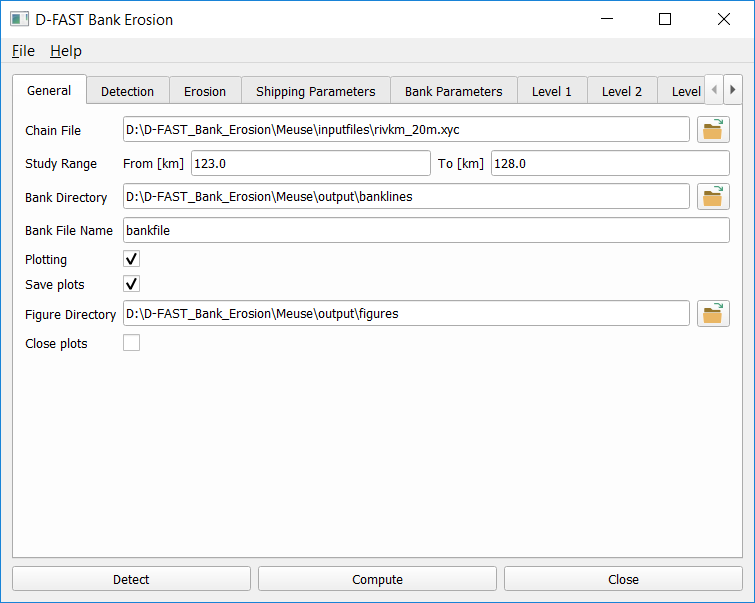
\includegraphics[width=\textwidth,height=11.4cm]{figures/gui1.png}
	\caption{Example of the General settings in the GUI. The explanation of these settings is given in \autoref{Sec:cfg}}
	\vspace*{-0.2cm} 
	\label{guiGeneral}
	\vspace*{-0.2cm} 
\end{figure}

\NumNote{All files and paths are shown using absolute paths in the graphical user interface, but they will be converted as much as possible to relative paths when saving the configuration to file.
The user interface does not verify or validate the content of the files.
This is only verified by the kernel during the analysis.}

\section{Run mode 'banklines'} \label{Sec:rundetect}

When \dfastbe is run in this mode, it determines the representative bank lines within the area of interest; for background information see \autoref{Chp:BankDetect}.
The input is given through the analysis configuration file, see \autoref{Sec:Prepare}.

When the configuration file has the name 'dfastbe.cfg' and is located in the work directory the program can be called as follows:

\begin{Verbatim}
dfastbe --mode banklines
\end{Verbatim}

If the definition file has another name the following call should be used:

\begin{Verbatim}
dfastbe --mode banklines --config D:\D-FAST_Bank_Erosion\Meuse\Meuse.cfg
\end{Verbatim}

with \command{path} the path to the directory where the configuration file is located and \command{other.cfg} the name of the configuration file.

Required input parameters:

\begin{itemize}
\item \dflowfm output file (netCDF map-file) at representative discharge (\command{SimFile}),
\item Number of bank Lines (\command{NBank} default two, the left and right bank),
\item For each of the bank lines a file with xy-coordinates of the search lines i.e. the approximate location of the bank line (\command{Line1}, \command{Line2}, ..., \command{LineN}, with $N$ the number of bank lines)
\item Chainage file which links river kilometres to xy-coordinates (\command{RiverKM}),
\end{itemize}

Output:

\begin{itemize}
\item XY-coordinates of the determined bank lines.
\item Plot of the bank lines (optional, \command{Plotting} and \command{SavePlots})
\end{itemize}

\begin{figure}[!b]
	\center
	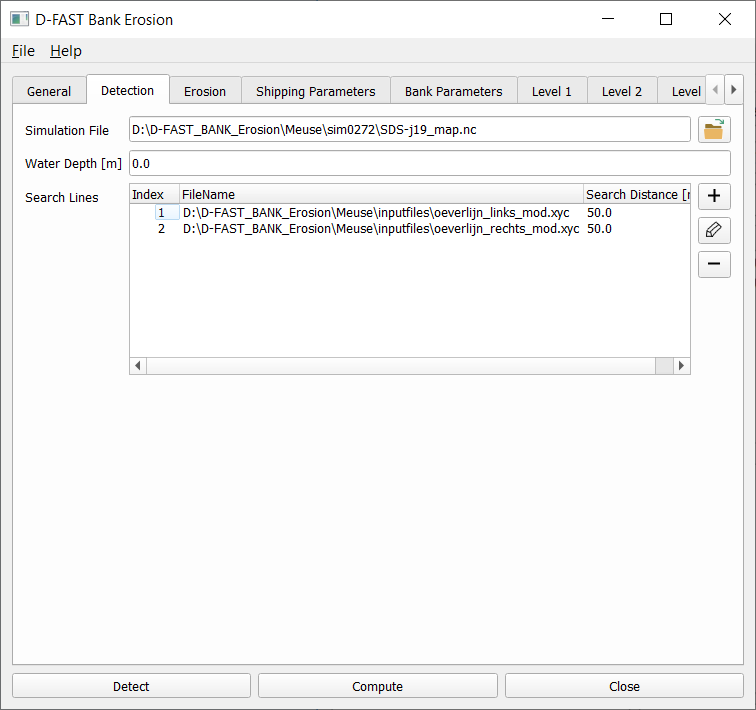
\includegraphics[width=\textwidth]{figures/gui2.png}
	\caption{Example of the Detection settings in the GUI. The settings are described in \autoref{Sec:cfg}}
	\label{guiDetect}
	\vspace*{-0.5cm} 
\end{figure}

\autoref{guiDetect} shows the tab in the graphical user interface for the settings specific for the detection step.
The content of the first (General) and second (Detection) tabs is relevant for the bank line detection analysis.
All files and paths are shown using absolute paths in the graphical user interface, but they will be converted as much as possible to relative paths when saving the configuration to file.
The user interface does not verify or validate the content of the files.
This is only verified by the kernel during the analysis.

An example of the graphical output of the 'banklines' mode is shown in \autoref{Fig2.2}.
The water depth is given with colored surfaces (per grid cell) clipped to the area close to the area of interest (about twice the maximum distance of the bank lines from the fairway), the black lines are the determined bank lines and the river kilometres are displayed along the river axis.
The computation has ended successfully when the message "BankLines ended successfully!" appears.
A full listing of the screen output of \dfastbe during the bank line detection analysis is given below at the end of this section in \autoref{logbanklines}. An example of the graphical output of the 'banklines' mode is shown in \autoref{Fig2.2}. In this figure the water depth is given with colored surfaces (per grid cell) clipped to the area close to the area of interest (about twice the maximum distance of the bank lines from the fairway), the black lines are the determined bank lines and the river kilometres are displayed along the river axis. 

\NumNote{It is advised to check the detected banklines shown in the graphical output of the 'banklines'mode before continuing with the 'bankerosion' mode. Common issues with bank line detection and their solutions are described in \autoref{Sec4.2}.}

\NumNote{To obtain the correct results, the search lines for the banks given by \command{Line1}, \command{Line2}, ..., \command{LineN} (obtained for example from the 'oeverlijnen' from Baseline data) should follow the actual bank line (to be detected) within a distance indicated by \command{DLines} (default 50 \unitbrackets{m}).
Large distances between the points -- and thus large deviations from the actual bank lines -- will result in inaccurate bank lines as the detection algorithm will not detect bank lines reaches outside the indicated area of interest.}

\NumNote{The chainage file containing the river kilometres should have sufficient resolution since the all data will be projected onto that line.
In the analysis, the reference points will be connected by straight lines with linearly interpolated chainage values.
It is suggested to provide all lines with at least the resolution of the simulation model from which the data is used, or at least every 100 m.}


\begin{figure}[!b]
\vspace*{-1cm} 
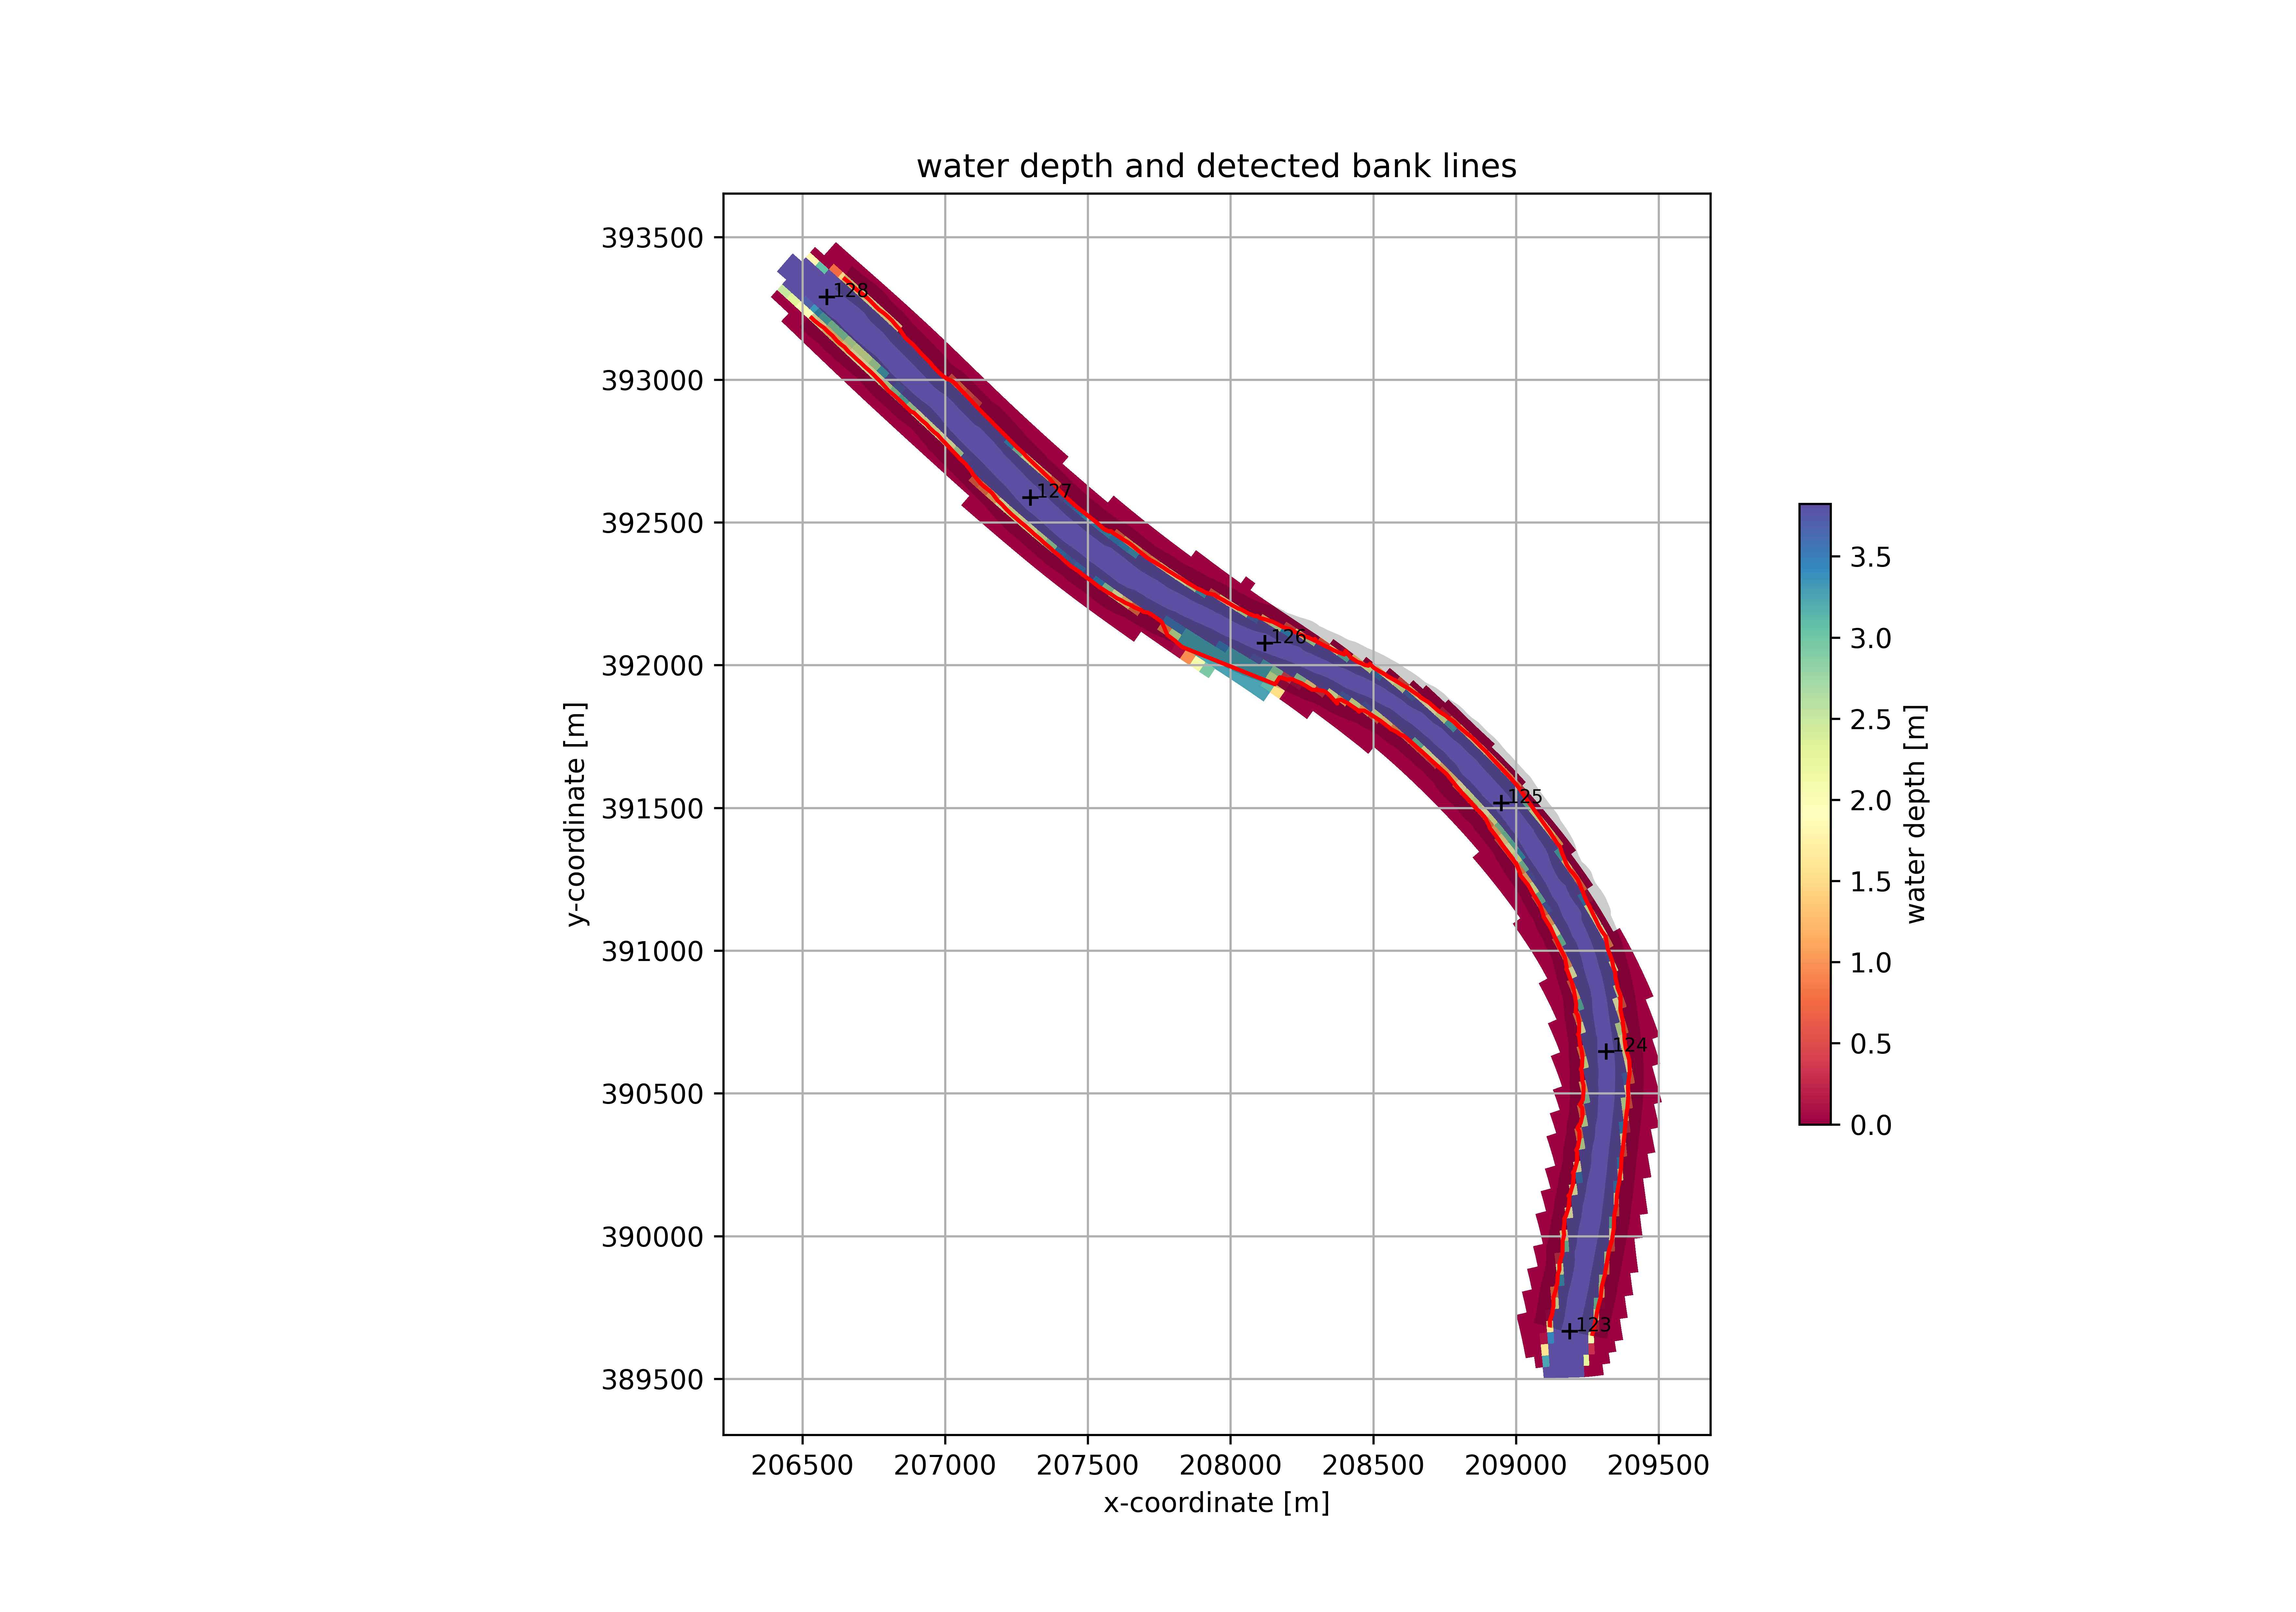
\includegraphics[width=\textwidth]{figures/1_banklinedetection.png}
\vspace*{-1cm} 
\caption{Example of output of \dfastbe in 'banklines' mode showing water depth, detected banklines (red lines), and river kilometres}
\label{Fig2.2}
\end{figure}

\pagebreak 

\begin{figure}[!ht]
\begin{Verbatim}
=====================================================
Determine bank lines
=====================================================
version: D-FAST Bank Erosion 2.1.0
source: https://github.com/Deltares/D-FAST_Bank_Erosion
-----------------------------------------------------
saving output in directory: output\banklines
WARNING: directory 'output\banklines' already exists...=> overwriting directory
saving figures in directory: output\figures
WARNING: directory 'output\figures' already exists...=> overwriting directory
reading chainage information from file : inputfiles\rivkm_20m.xyc
clipping chainage to the range 123.0 to 128.0 km
reading search line 1 from file : inputfiles\oeverlijn_links_mod.xyc
reading search line 2 from file : inputfiles\oeverlijn_rechts_mod.xyc
-----------------------------------------------------
reading simulation data from : sim270\SDS-j19_map.nc
-----------------------------------------------------
importing grid...
importing bathymetry ...
importing water level ...
importing water depth ...
importing velocity ...
importing Chezy ...
importing dry/wet information ...
-----------------------------------------------------
clipping simulation data to area of interest ...
defining coordinates of bank lines ...
0%
10%
20%
30%
40%
50%
60%
70%
80%
90%
100%
clipping, sorting and connecting bank lines ...
- bank line 1
- bank line 2
-----------------------------------------------------
saving bank lines to file: output\banklines\bankfile.shp
=====================================================
generating figures ...
saving figure output\figures\1_banklinedetection.png

=====================================================
===    Bank line detection ended successfully!    ===
=====================================================
\end{Verbatim}
\caption{Example of the log for of \dfastbe in 'banklines' mode}
\label{logbanklines}
\end{figure}

\pagebreak 

\section{Run mode 'bankerosion'} \label{Sec:runerosion}

When \dfastbe is run in this mode, it determines the expected bank erosion within the area of interest; for background information see \autoref{Chp:BankErosion}.
The input is given through the analysis configuration file, see \autoref{Sec:Prepare}.

When the configuration file has the name 'dfastbe.cfg' and is located in the work directory the program can be called as follows:

\begin{Verbatim}
dfastbe --mode bankerosion
\end{Verbatim}

If the configuration file has another name the following call should be used:

\begin{Verbatim}
dfastbe --mode bankerosion --config D:\D-FAST_Bank_Erosion\Meuse\Meuse.cfg
\end{Verbatim}

with \command{path} the path to the directory where the configuration file is located and \command{other.cfg} the name of the configuration file.

Required input:

\begin{itemize}
\item The period during which the bank erosion acts (\command{TErosion}, default 1 year),
\item The number of discharge levels (\command{NLevel}),
\item \dflowfm files (netCDF map-files) for the different discharge levels and the corresponding probability distribution (\command{SimFile1}, \command{SimFile2}, ..., \command{FileN} and \command{PDischarge1}, \command{PDischarge2}, ..., \command{PDischargeN}, with $N$ the number of discharge levels),
\item Number of bank lines (\command{Nbank} default 2: the left and right bank),
\item File which links river chainage (kilometres) to xy-coordinates (\command{RiverKM}),
\item XY-coordinates of the river and fairway axis (\command{RiverAxis}, \command{Fairway}),
\item Information about the strength or type of the soil of the banks (\command{BankType}).
This can be done either in the form of classes or with a critical shear stress (see \autoref{Tab4.1}).
In the first case \command{Classes} should be set to \command{true} and in the second case to \command{false} (default).
The bank strength information can be given either as a constant value for the whole track or as a river kilometre dependent quantity in a ASCII-file per bank (see \autoref{Sec:parfile}),
\item Shipping information (\command{Vship}, \command{Nship}, \command{ShipType}, \command{Draught}).
This can again be given either as a constant value for the whole track or as a river kilometre dependent quantity in a single ASCII-file (see \autoref{Sec:parfile}).
\end{itemize}

\NumNote{The chainage file and the river and fairway axis files should be provided with sufficient resolution.
\dfastbe will use straight lines between the specified reference points which deviates from the natural curved channel planform.
It is, therefore, suggested to provide all lines with at least the resolution of the simulation model from which the data is used, or at least every 100 m.}

\NumNote{Even if default values or default files have been provided for input parameters, the user always needs to show whether those inputs given are appropriate for the intended application.}

The settings for the bank erosion analysis are distributed over several tabs.
All tabs except for the second (Detection) tab are relevant for the bank erosion analysis.
First of all, \autoref{guiErode} shows the main settings for the erosion step such as the simulation period, the simulations and the associated weights.
Subsequently, there are tabs for the shipping parameters (\autoref{guiShip}), bank parameters (\autoref{guiBank}) and shipping and bank parameters that may vary per discharge level (\autoref{guiLevelX}).
All quantities in the first two parameter tabs must be specified either as constants or as file based (described in \autoref{Sec:parfile}).
The quantities in the other level parameters tabs are optional; by default they will set to "Use Default" which means use the (discharge level independent) value(s) specified in the first two tabs.
All files and paths are shown using absolute paths in the graphical user interface, but they will be converted as much as possible to relative paths when saving the configuration to file.
The user interface does not verify or validate the content of the files.
This is only verified by the kernel during the analysis.


\NumNote{When specifying chainage dependent values for \keyw{Slope}, \keyw{Reed}, \keyw{BankType} and \keyw{ProtectionLevel}, please follow the file name conventions listed in \autoref{Sec:parfile}.}

\begin{figure}[!h]
	\center 
	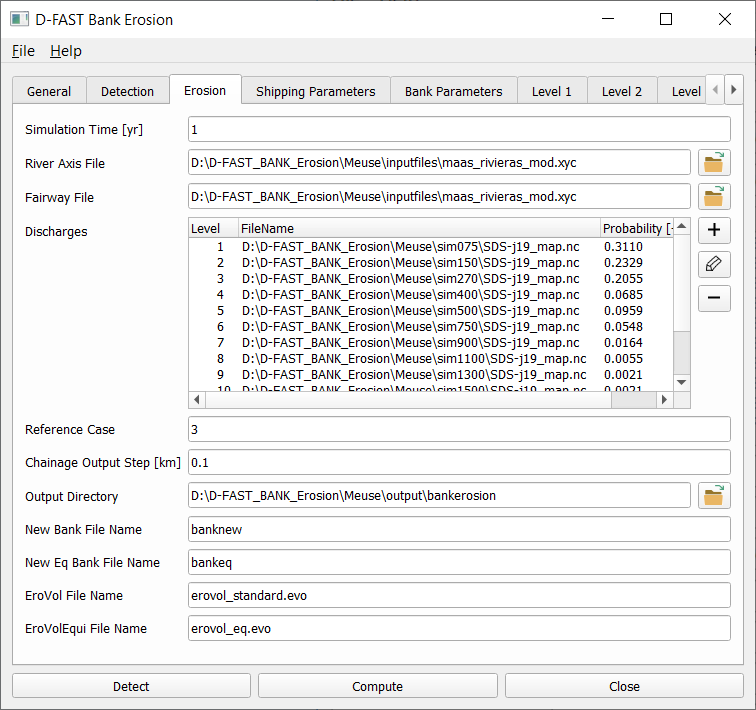
\includegraphics[width=\textwidth,height=11.4cm]{figures/gui3.png}
	\caption{Example of the Erosion settings in the GUI.The settings are described in \autoref{Sec:cfg}}
	\label{guiErode}
\end{figure}


\clearpage
\begin{figure}[!ht]
\center
\vspace{-0.75cm} 
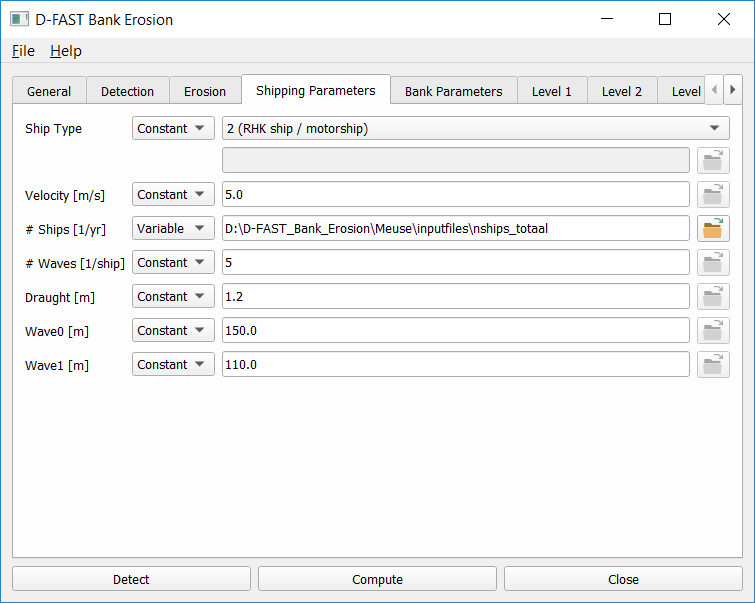
\includegraphics[width=\textwidth,height=11.2cm]{figures/gui4.png}
\caption{Example of the Shipping Parameters in the GUI. The parameters are described in \autoref{Sec:cfg} and in section in \autoref{Sec:parfile} for chainage dependent values.}
\label{guiShip}
\end{figure}

\begin{figure}[!hb]
\center
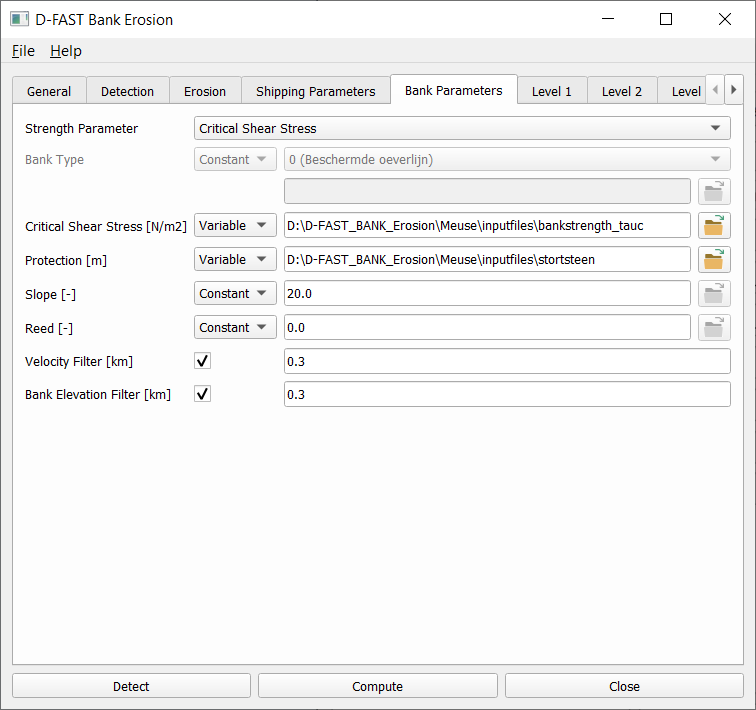
\includegraphics[width=\textwidth,height=11.2cm]{figures/gui5.png}
\caption{Example of the Bank Parameters in the GUI}
\vspace{-0.75cm} 
\label{guiBank}

\end{figure}

\clearpage
\begin{figure}[!ht]
\vspace{-0.75cm} 
\center
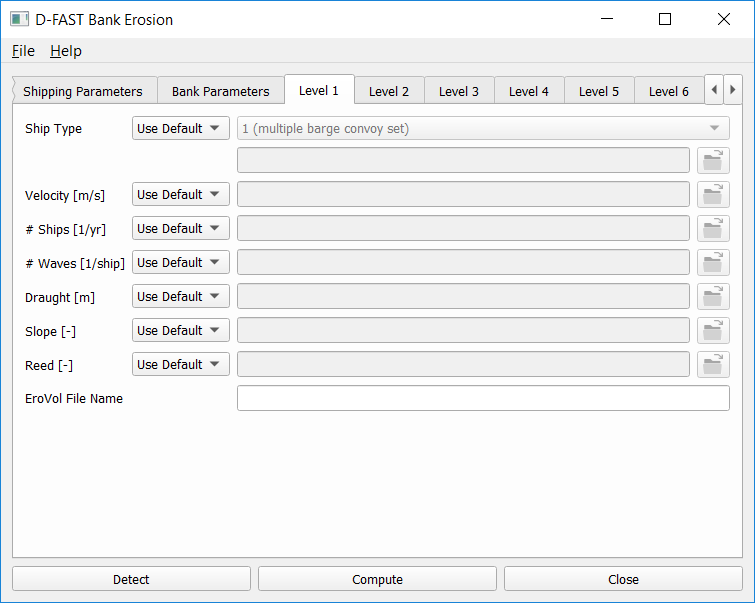
\includegraphics[width=\textwidth,height=11.4cm]{figures/gui6.png}
\caption{Example of the Discharge Level dependent parameters in the GUI, which are described in \autoref{Sec:cfg}}
\label{guiLevelX}
\vspace{-0.15cm} 
\end{figure}

Output:

\begin{itemize}
	\item Map with water depth, initial bank lines, river kilometres and fairway axis (see \autoref{Fig2.4}),
	\item Map with erosion sensitivity of the banks based on computed bank retreat (see \autoref{Fig2.5}),
	\item The computed erosion volume during the simulation period split up per discharge level (see \autoref{Fig2.6a}) and per bank (see \autoref{Fig2.6b}),
	\item Total erosion volume based on equilibrium bank line (see \autoref{Fig2.7}),
	\item Control figures for water levels of each discharge (see \autoref{Fig2.8} and \autoref{Fig2.9}),
	\item Control figures for flow velocity of each discharge (see \autoref{Fig2.10} and \autoref{Fig2.11}),
	\item Map with indication of applied bank type (see \autoref{Fig2.12}),
	\item Bank retreat at the end of the simulation period and for the equilibrium situation (see \autoref{Fig2.13}),
	\item XY-coordinates of the computed bank lines at the end of the simulation period and of the equilibrium bank lines.
\end{itemize}

The maps and graphs are only created when \command{Plotting} is on and written to file if \command{SavePlots} is on.
You may optionally request zoomed versions of these plots by switching on \command{SaveZoomPlots} and selecting the desired step size for the chainage.
The computation has ended successfully when the message "Bank line detection ended successfully!" appears.
The listing of the screen output of \dfastbe during the bank erosion analysis is given below.

\newpage
\begin{Verbatim}
	=====================================================
	Compute bank erosion
	=====================================================
	version: D-FAST Bank Erosion 2.1.0
	source: https://github.com/Deltares/D-FAST_Bank_Erosion
	-----------------------------------------------------
	getting input from directory: output\banklines
	saving output in directory: output\bankerosion
	WARNING: directory 'output\bankerosion' already exists...=> overwriting directory
	saving figures in directory: output\figures
	WARNING: directory 'output\figures' already exists...=> overwriting directory
	total simulation time: 1.00 year
	-----------------------------------------------------
	reading simulation data from : sim075\SDS-j19_map.nc
	-----------------------------------------------------
	importing grid...
	importing bathymetry ...
	importing water level ...
	importing water depth ...
	importing velocity ...
	importing Chezy ...
	importing dry/wet information ...
	-----------------------------------------------------
	deriving mesh topology arrays ...
	reading chainage information from file : inputfiles\rivkm_20m.xyc
	clipping chainage to the range 123.0 to 128.0 km
	reading bank lines from file: output\banklines\bankfile.shp
	intersect bank lines with mesh ...
	- bank line 1 (244 nodes)
	- bank line 2 (263 nodes)
	mapping chainage to bank segments ...
	- bank line 1 on the left
	- bank line 2 on the right
	reading location of river axis from file: inputfiles\maas_rivieras_mod.xyc
	selecting river axis range of interest ...
	reading location of fairway from file: inputfiles\maas_rivieras_mod.xyc
	selecting fairway range of interest ...
	intersect fairway with mesh (362 nodes) ...
	computing distance between bank lines and fairway ...
	reading NShip from file: inputfiles\nships_totaal
	reading BankType of bank 1 from file: inputfiles\bankstrength_tauc_1.btp
	reading BankType of bank 2 from file: inputfiles\bankstrength_tauc_2.btp
	reading ProtectionLevel of bank 1 from file: inputfiles\stortsteen_1.bpl
	reading ProtectionLevel of bank 2 from file: inputfiles\stortsteen_2.bpl
	processing level information ...
	#####################
	### Discharge   1 ###
	#####################
	Discharge probability: 0.31
	Simulation time: 0.31 year
	reading level specific parameters ...
	-----------------------------------------------------
	reading simulation data from : sim075\SDS-j19_map.nc
	-----------------------------------------------------
	importing grid...
	importing bathymetry ...
	importing water level ...
	importing water depth ...
	importing velocity ...
	importing Chezy ...
	importing dry/wet information ...
	-----------------------------------------------------
	computing bank erosion ...
	saving eroded volume in file: erovolQ1.evo
	
	---- repetitive mid section skipped ----
	
	#####################
	### Discharge  13 ###
	#####################
	Discharge probability: 0.00
	Simulation time: 0.00 year
	reading level specific parameters ...
	-----------------------------------------------------
	reading simulation data from : sim2300\SDS-j19_map.nc
	-----------------------------------------------------
	importing grid...
	importing bathymetry ...
	importing water level ...
	importing water depth ...
	importing velocity ...
	importing Chezy ...
	importing dry/wet information ...
	-----------------------------------------------------
	computing bank erosion ...
	saving eroded volume in file: erovolQ13.evo
	=====================================================
	average erosion distance for bank line  1 :   0.15 m
	average erosion distance through flow     :   0.05 m
	average erosion distance through ships    :   0.10 m
	maximum erosion distance                  :   0.64 m
	average equilibrium erosion distance      :  11.59 m
	maximum equilibrium erosion distance      :  14.02 m
	-----------------------------------------------------
	average erosion distance for bank line  2 :   1.25 m
	average erosion distance through flow     :   0.62 m
	average erosion distance through ships    :   0.63 m
	maximum erosion distance                  :   4.59 m
	average equilibrium erosion distance      :  12.69 m
	maximum equilibrium erosion distance      :  14.52 m
	saving bank lines to file: output\bankerosion\bankfile_new.shp
	saving bank lines to file: output\bankerosion\bankfile_eq.shp
	saving total eroded volume in file: erovol_standard.evo
	saving equilibrium eroded volume in file: erovol_eq.evo
	=====================================================
	generating figures ...
	saving figure output\figures\1_banklines.png
	saving figure output\figures\2_erosion_sensitivity.png
	saving figure output\figures\3_eroded_volume_per_discharge.png
	saving figure output\figures\4_eroded_volume_per_bank.png
	saving figure output\figures\5_eroded_volume_eq.png
	saving figure output\figures\6_levels_bank_1.png
	saving figure output\figures\7_levels_bank_2.png
	saving figure output\figures\8_velocity_bank_1.png
	saving figure output\figures\9_velocity_bank_2.png
	saving figure output\figures\10_banktype.png
	saving figure output\figures\11_erodis.png
	
	=====================================================
	===   Bank erosion analysis ended successfully!   ===
	=====================================================
\end{Verbatim}
\begin{figure}[!h]
	\caption{Example of the log for of \dfastbe in 'bankerosion' mode}
	\label{logbankerosion}
\end{figure}

\clearpage
\begin{figure}
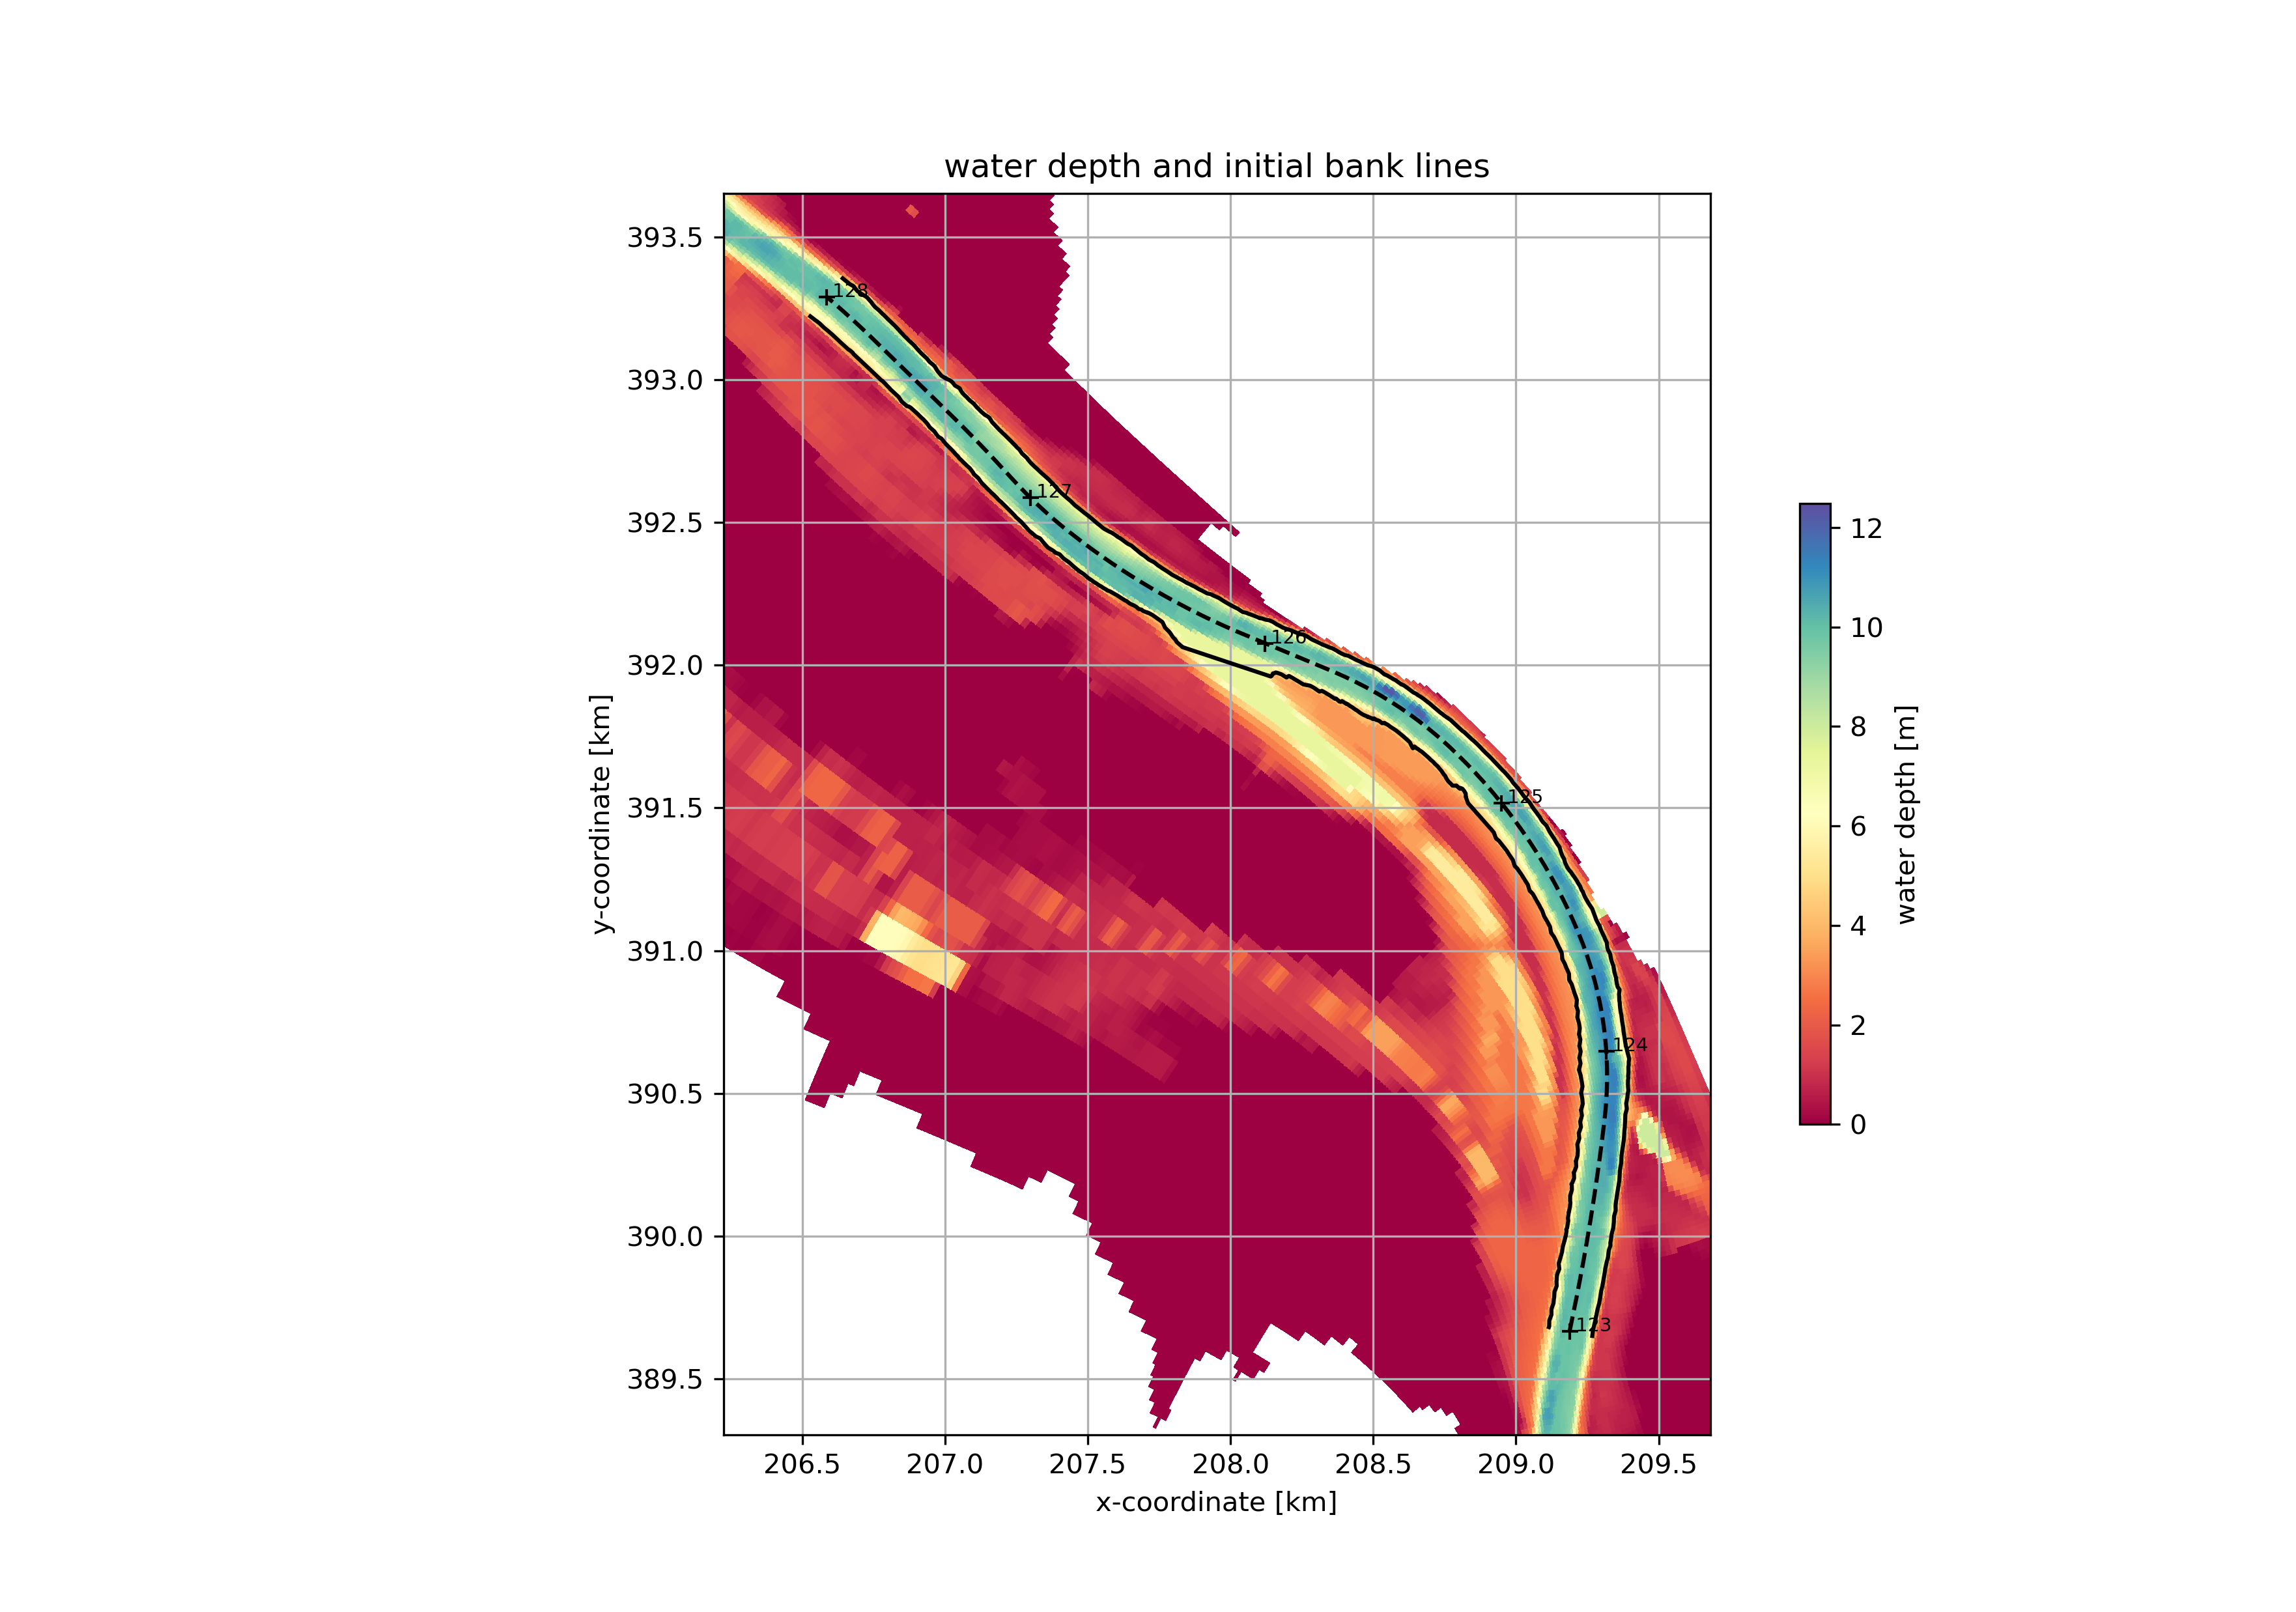
\includegraphics[width=\textwidth]{figures/1_banklines.png}
\caption{Map of water depth, initial bank lines, river kilometres and fairway axis}
\label{Fig2.4}
\end{figure}

\begin{figure}
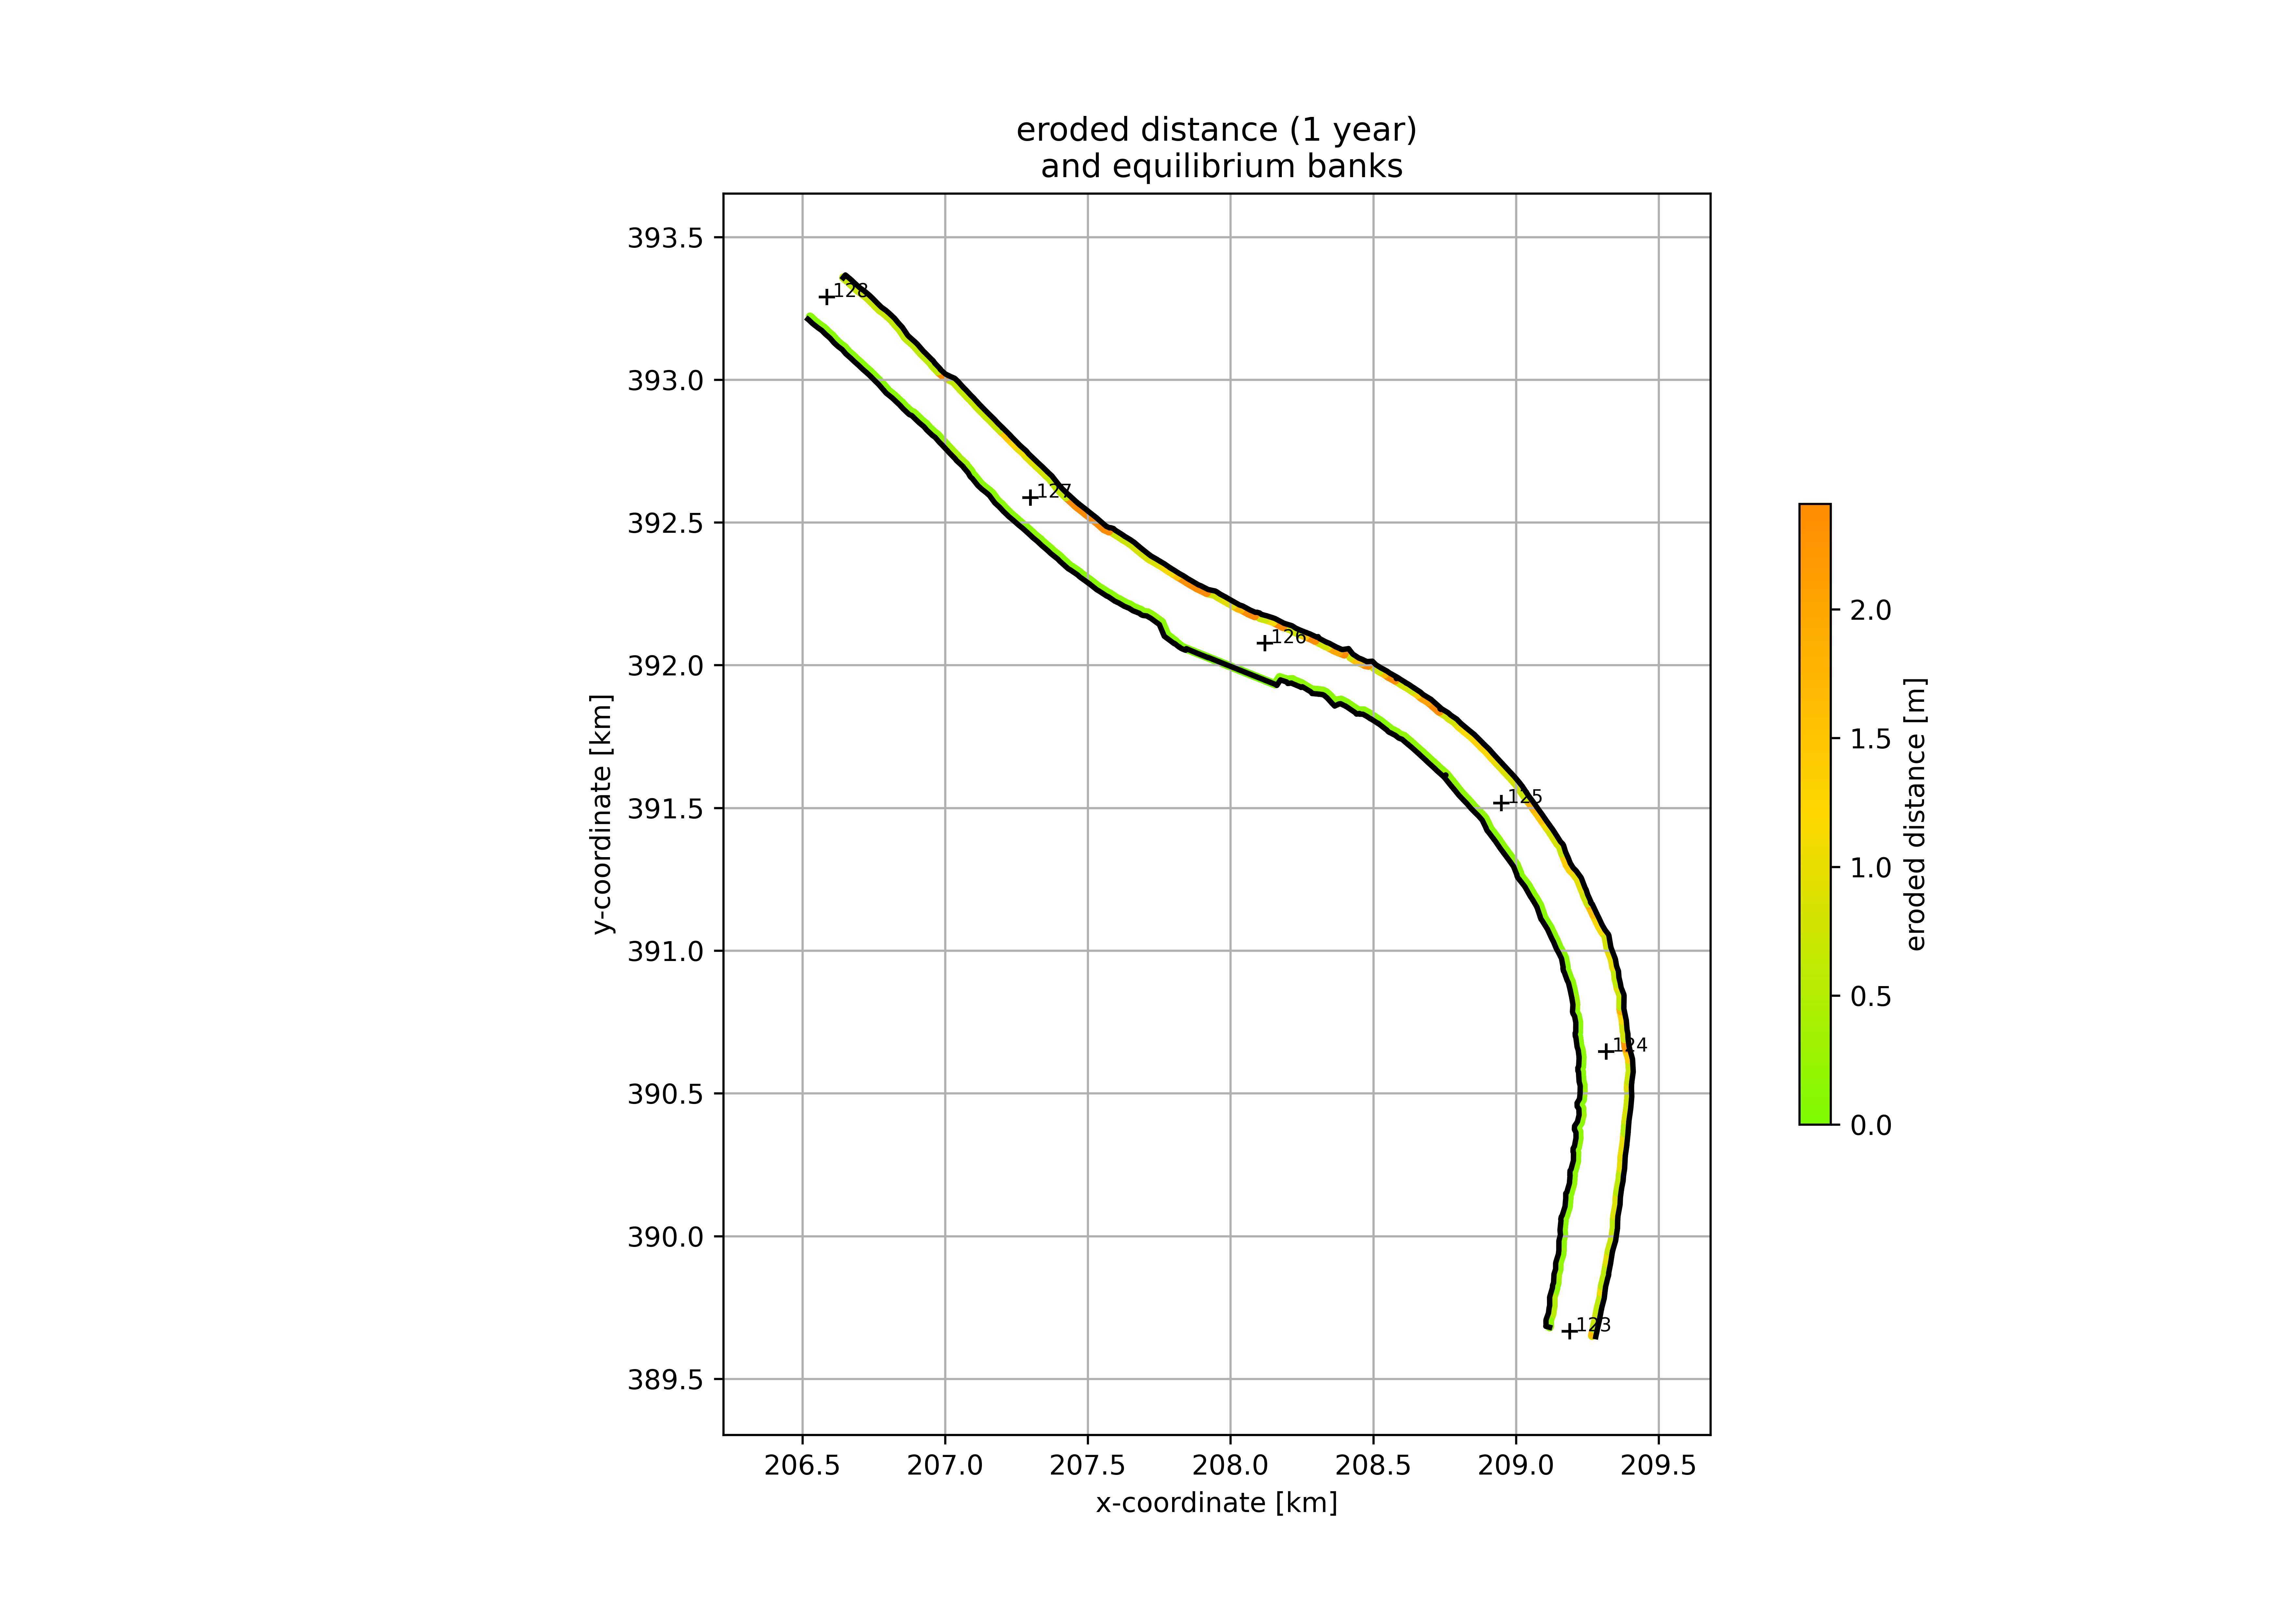
\includegraphics[width=\textwidth]{figures/2_erosion_sensitivity.png}
\caption{Map of erosion sensitivity}
\label{Fig2.5}
\end{figure}

\clearpage
\begin{figure}
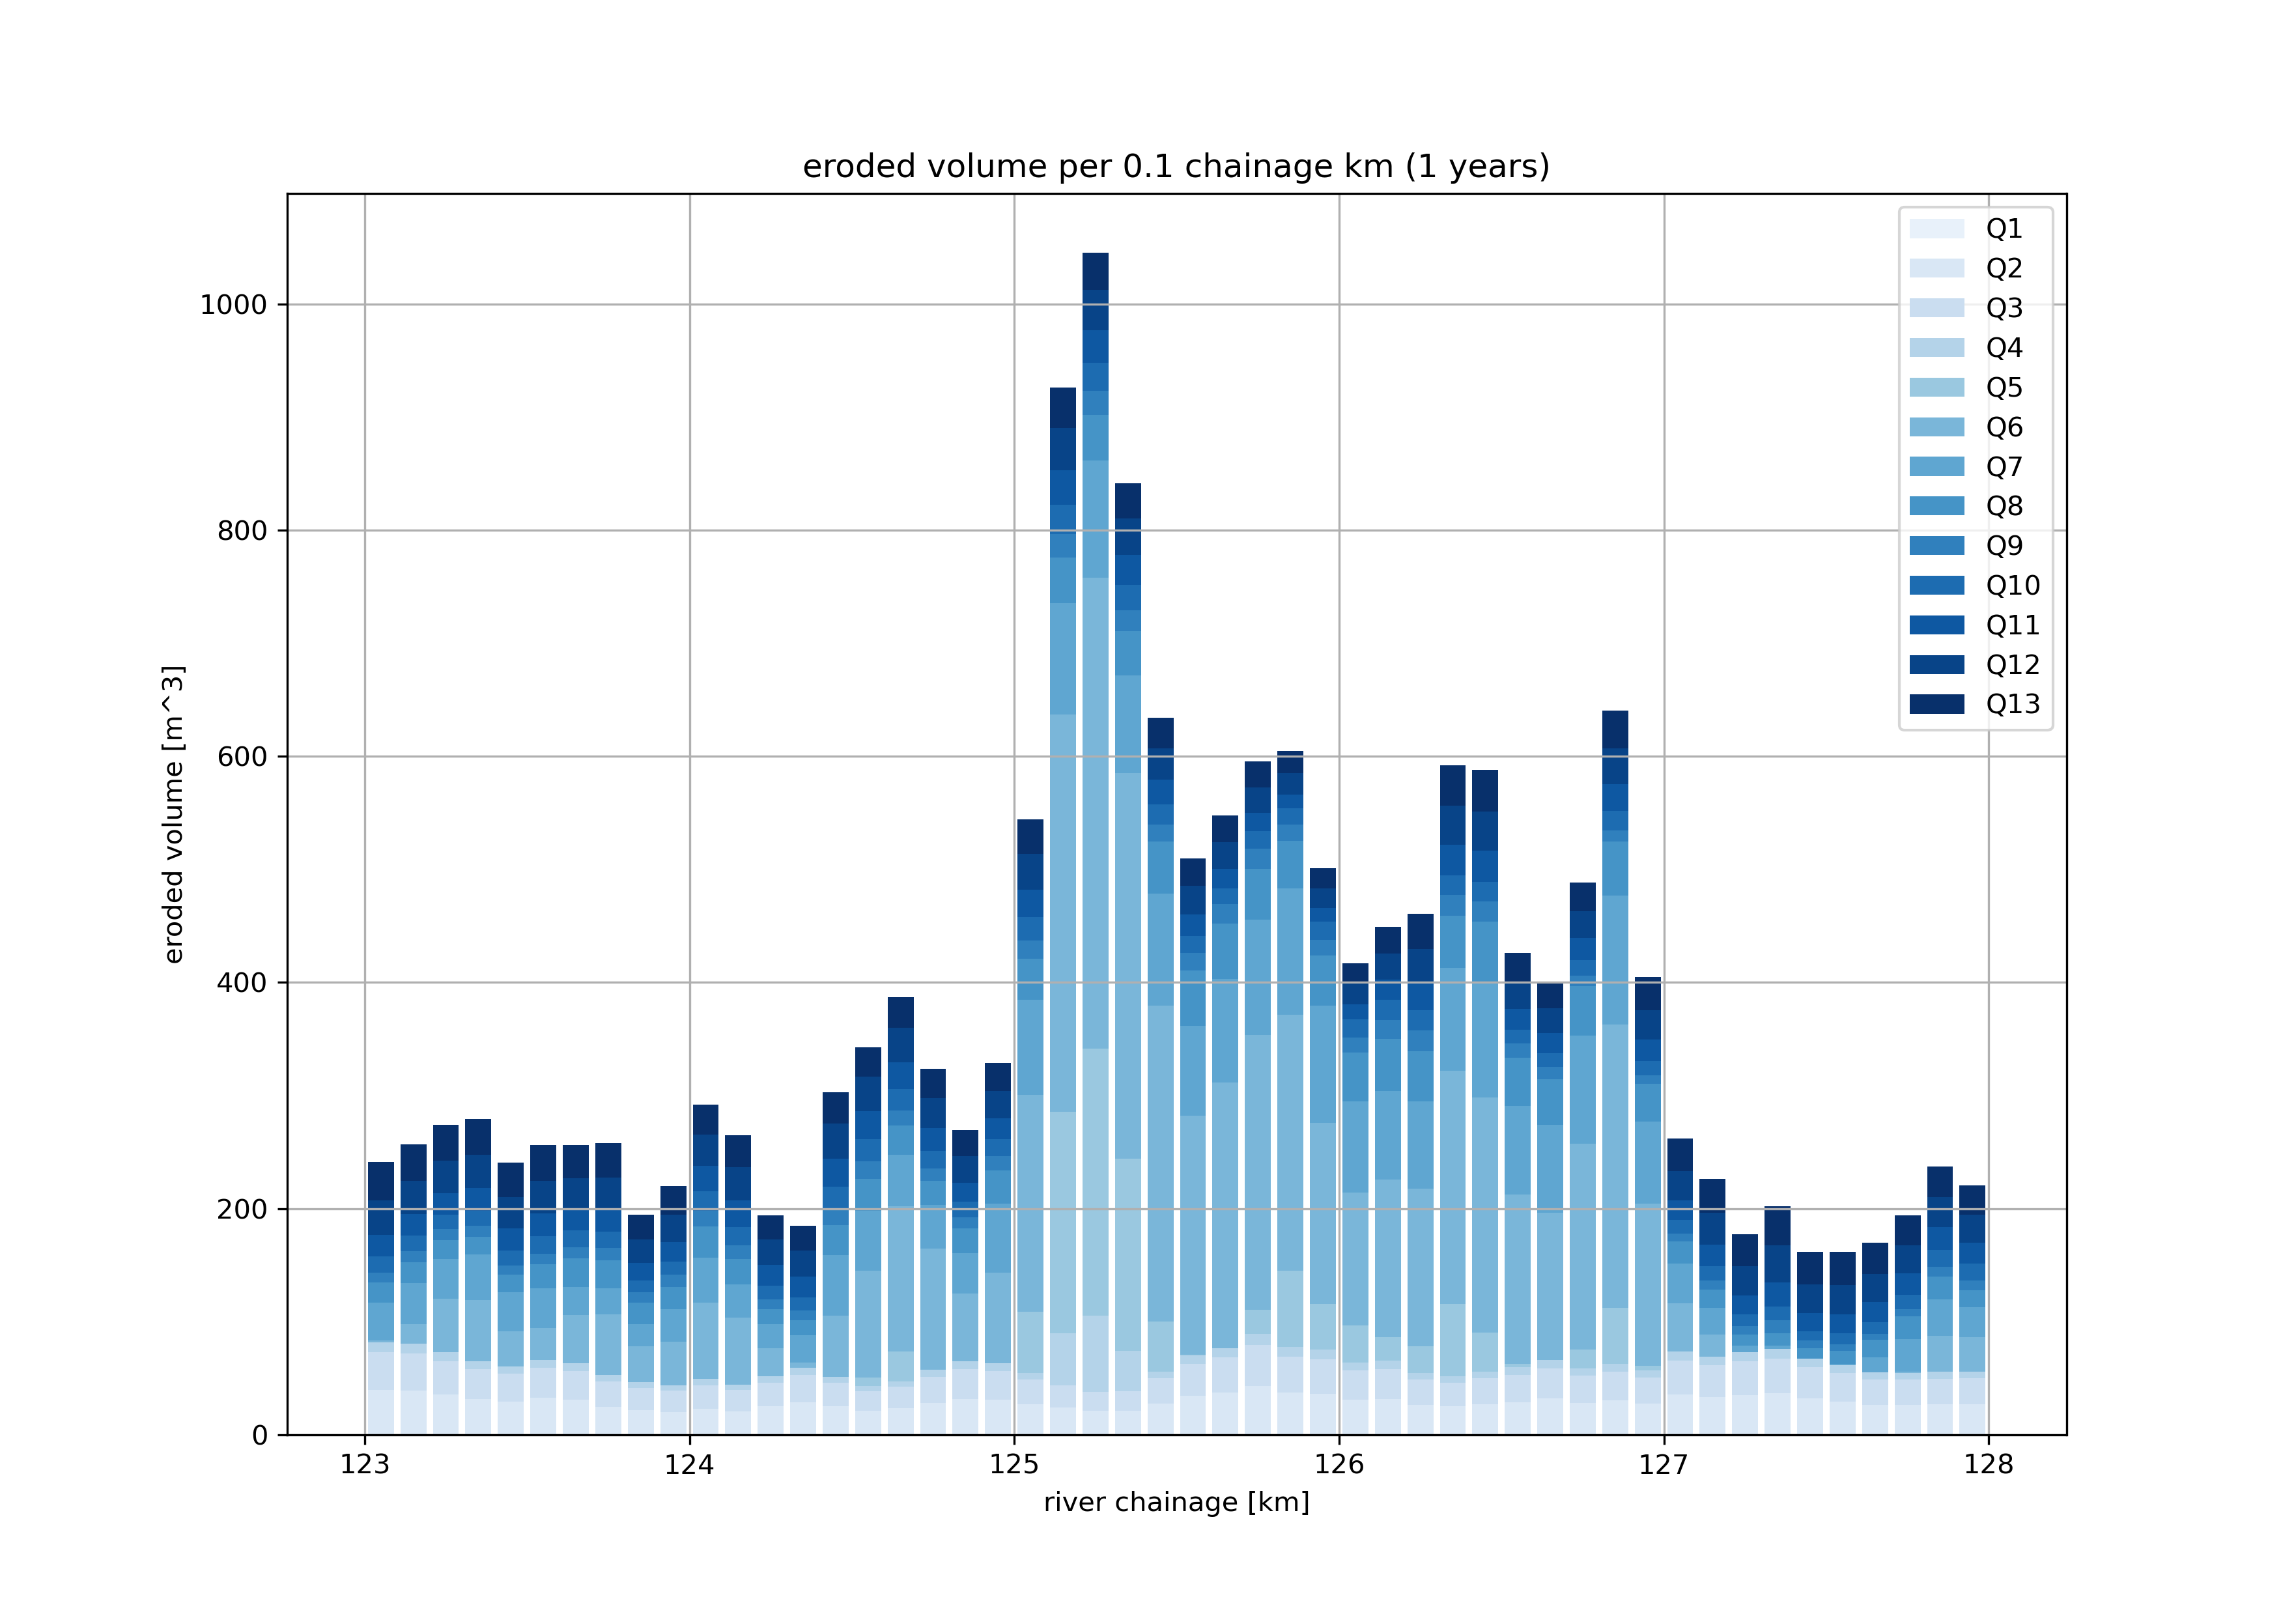
\includegraphics[width=\textwidth]{figures/3_eroded_volume_per_discharge.png}
\caption{Eroded volume subdivided per discharge level}
\label{Fig2.6a}
\end{figure}

\begin{figure}
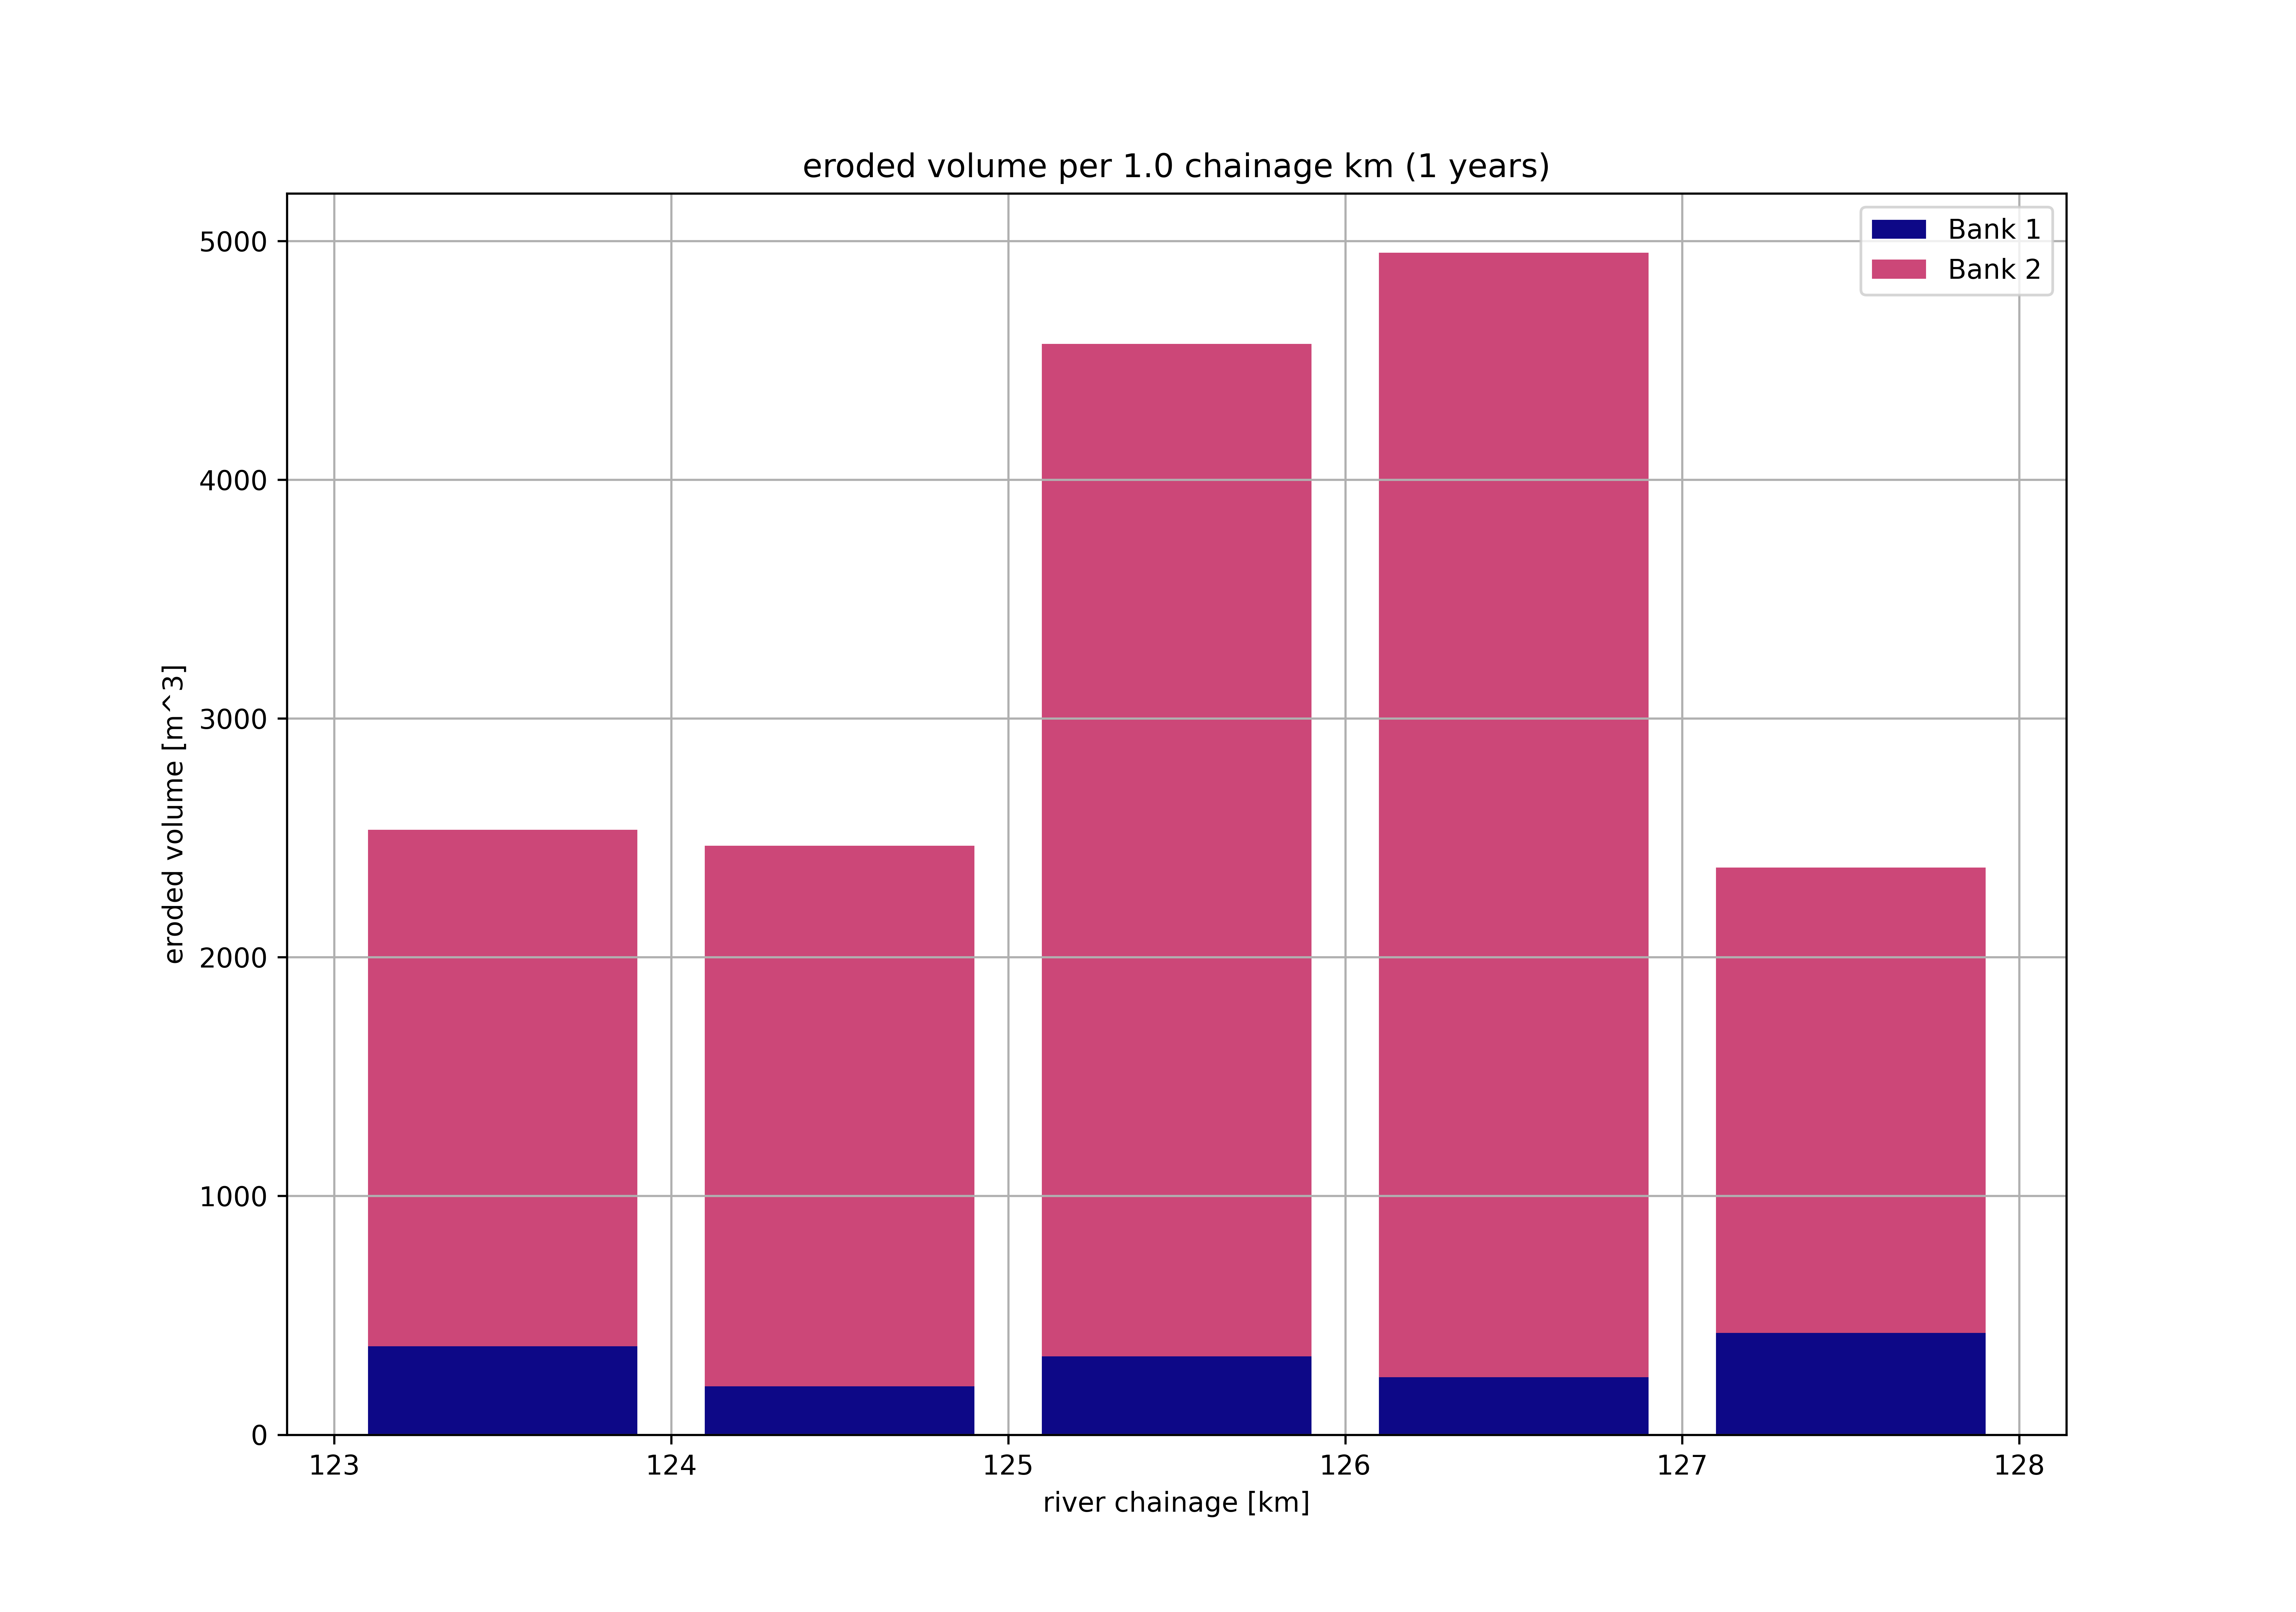
\includegraphics[width=\textwidth]{figures/4_eroded_volume_per_bank.png}
\caption{Eroded volume subdivided per bank line}
\label{Fig2.6b}
\end{figure}
\clearpage
\begin{figure}
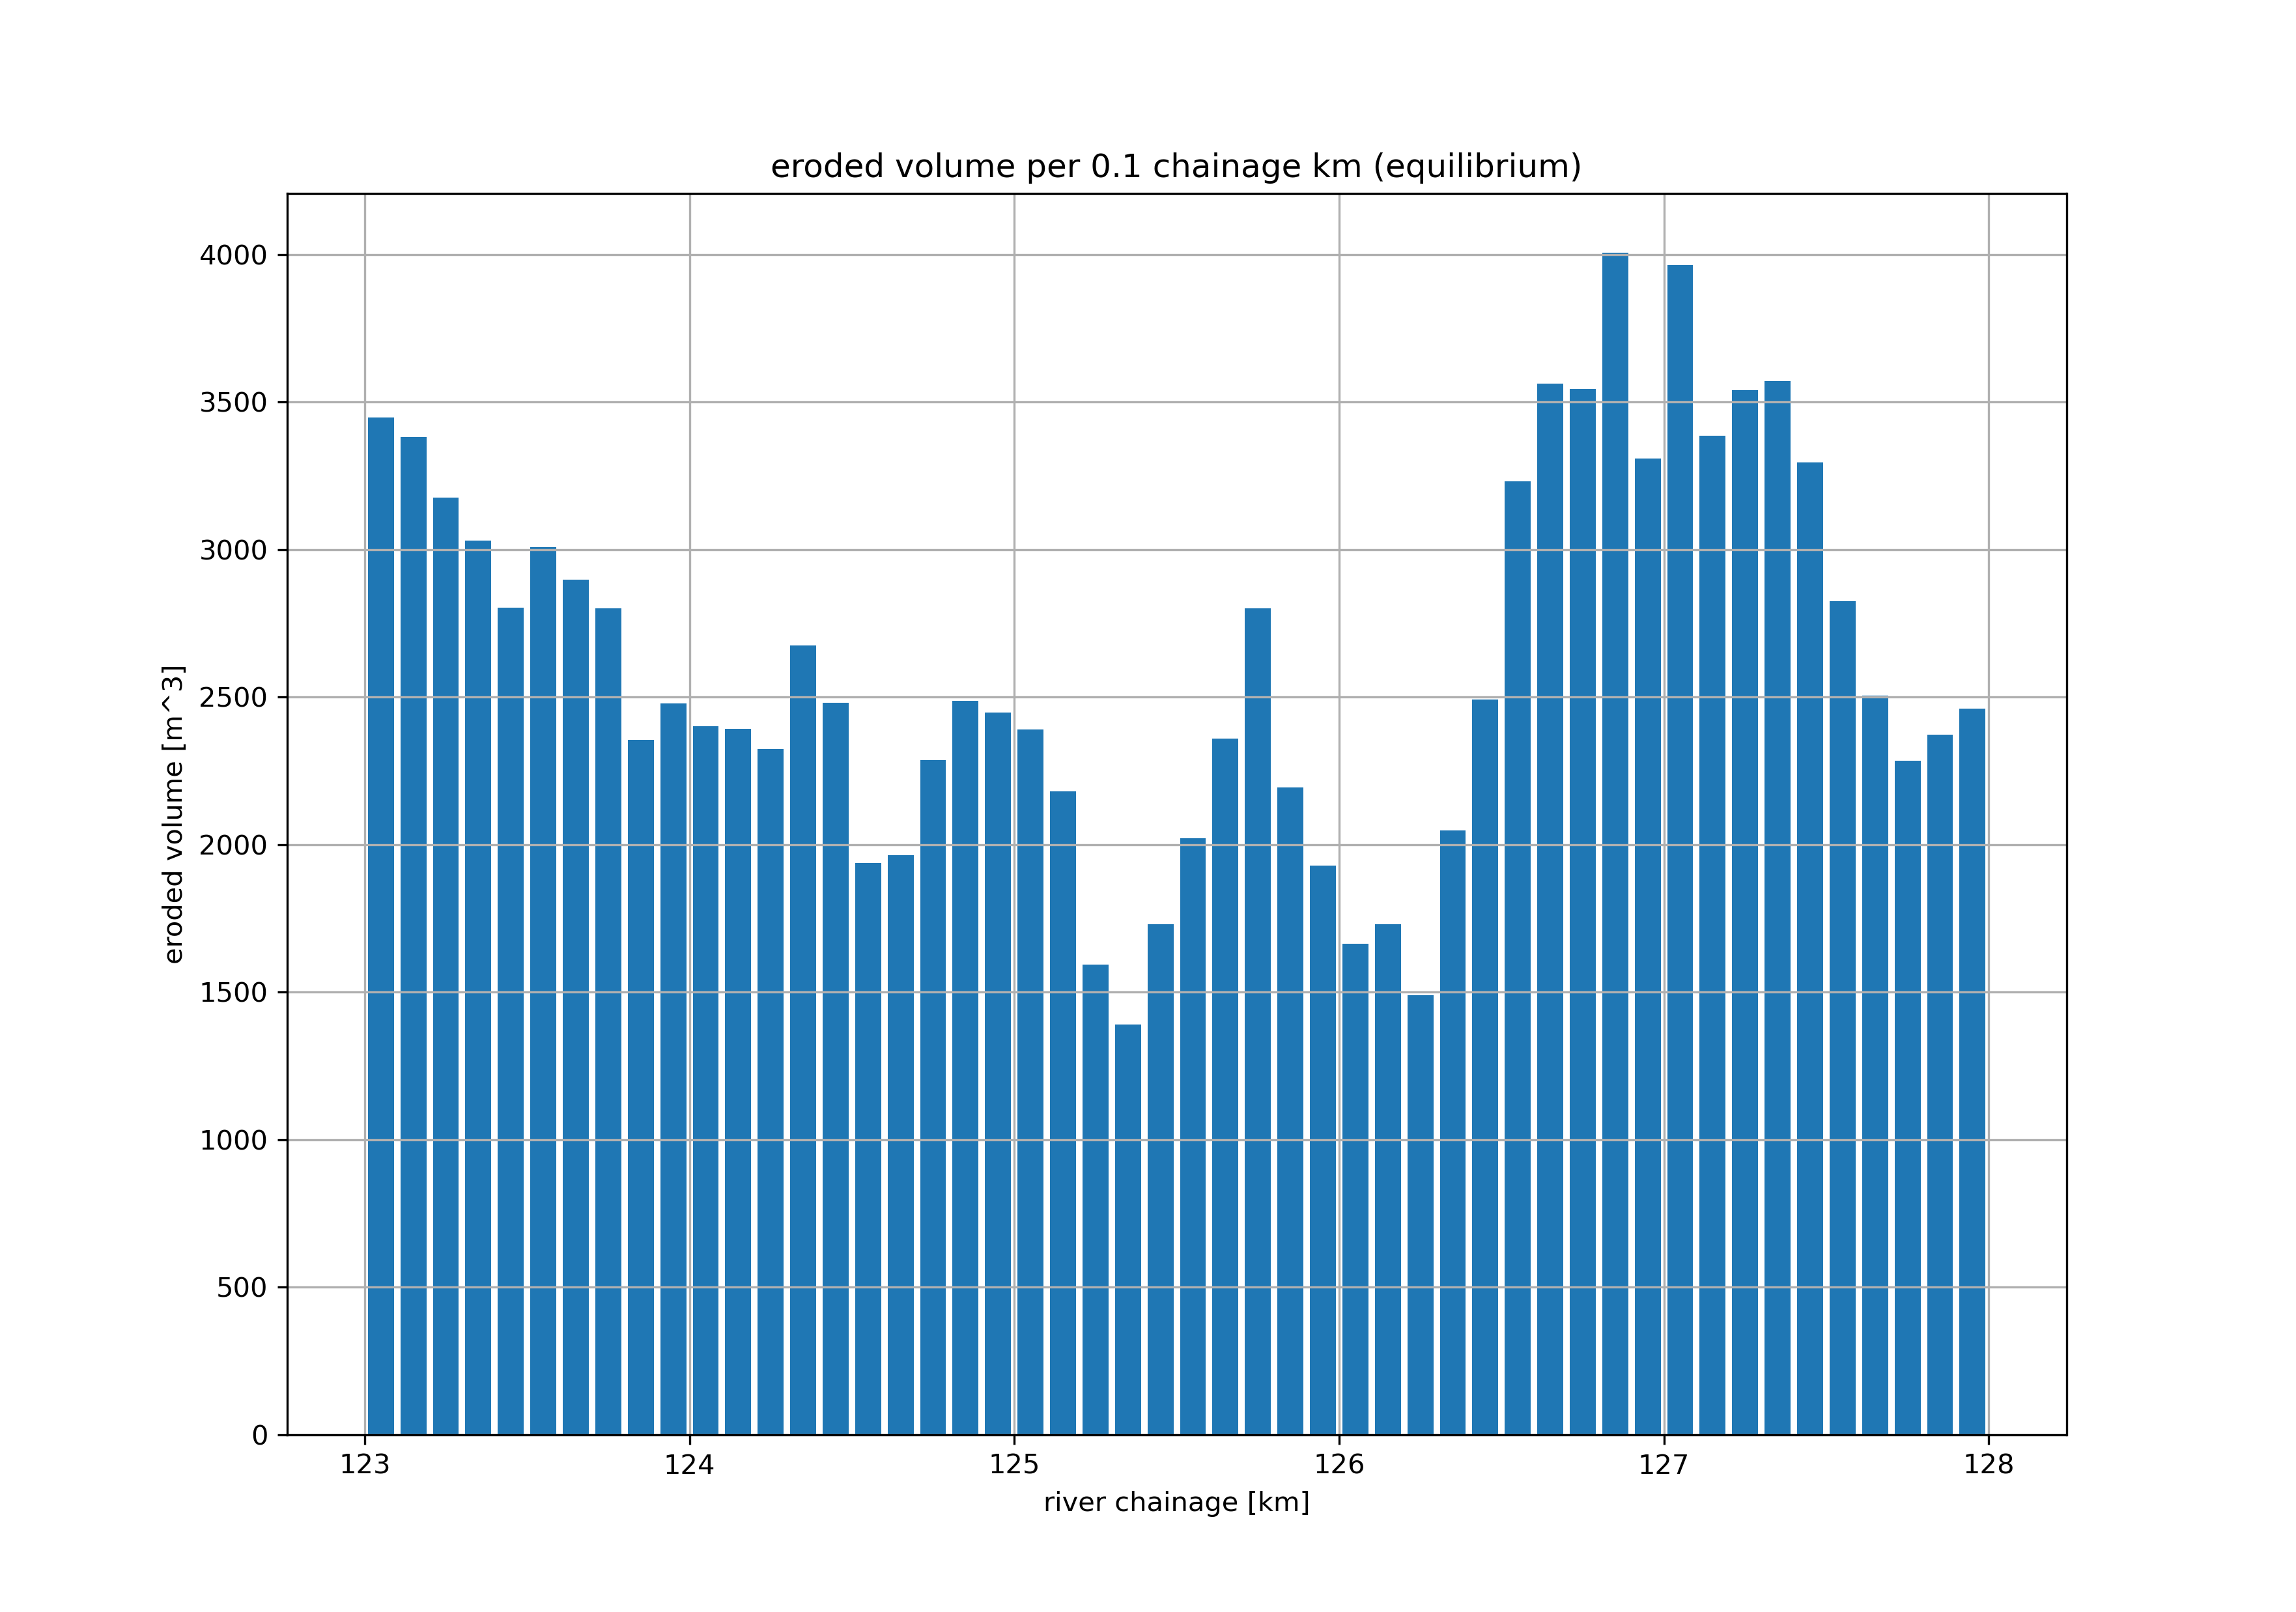
\includegraphics[width=\textwidth]{figures/5_eroded_volume_eq.png}
\caption{Total erosion volume based on equilibrium bank line}
\label{Fig2.7}
\end{figure}

\begin{figure}
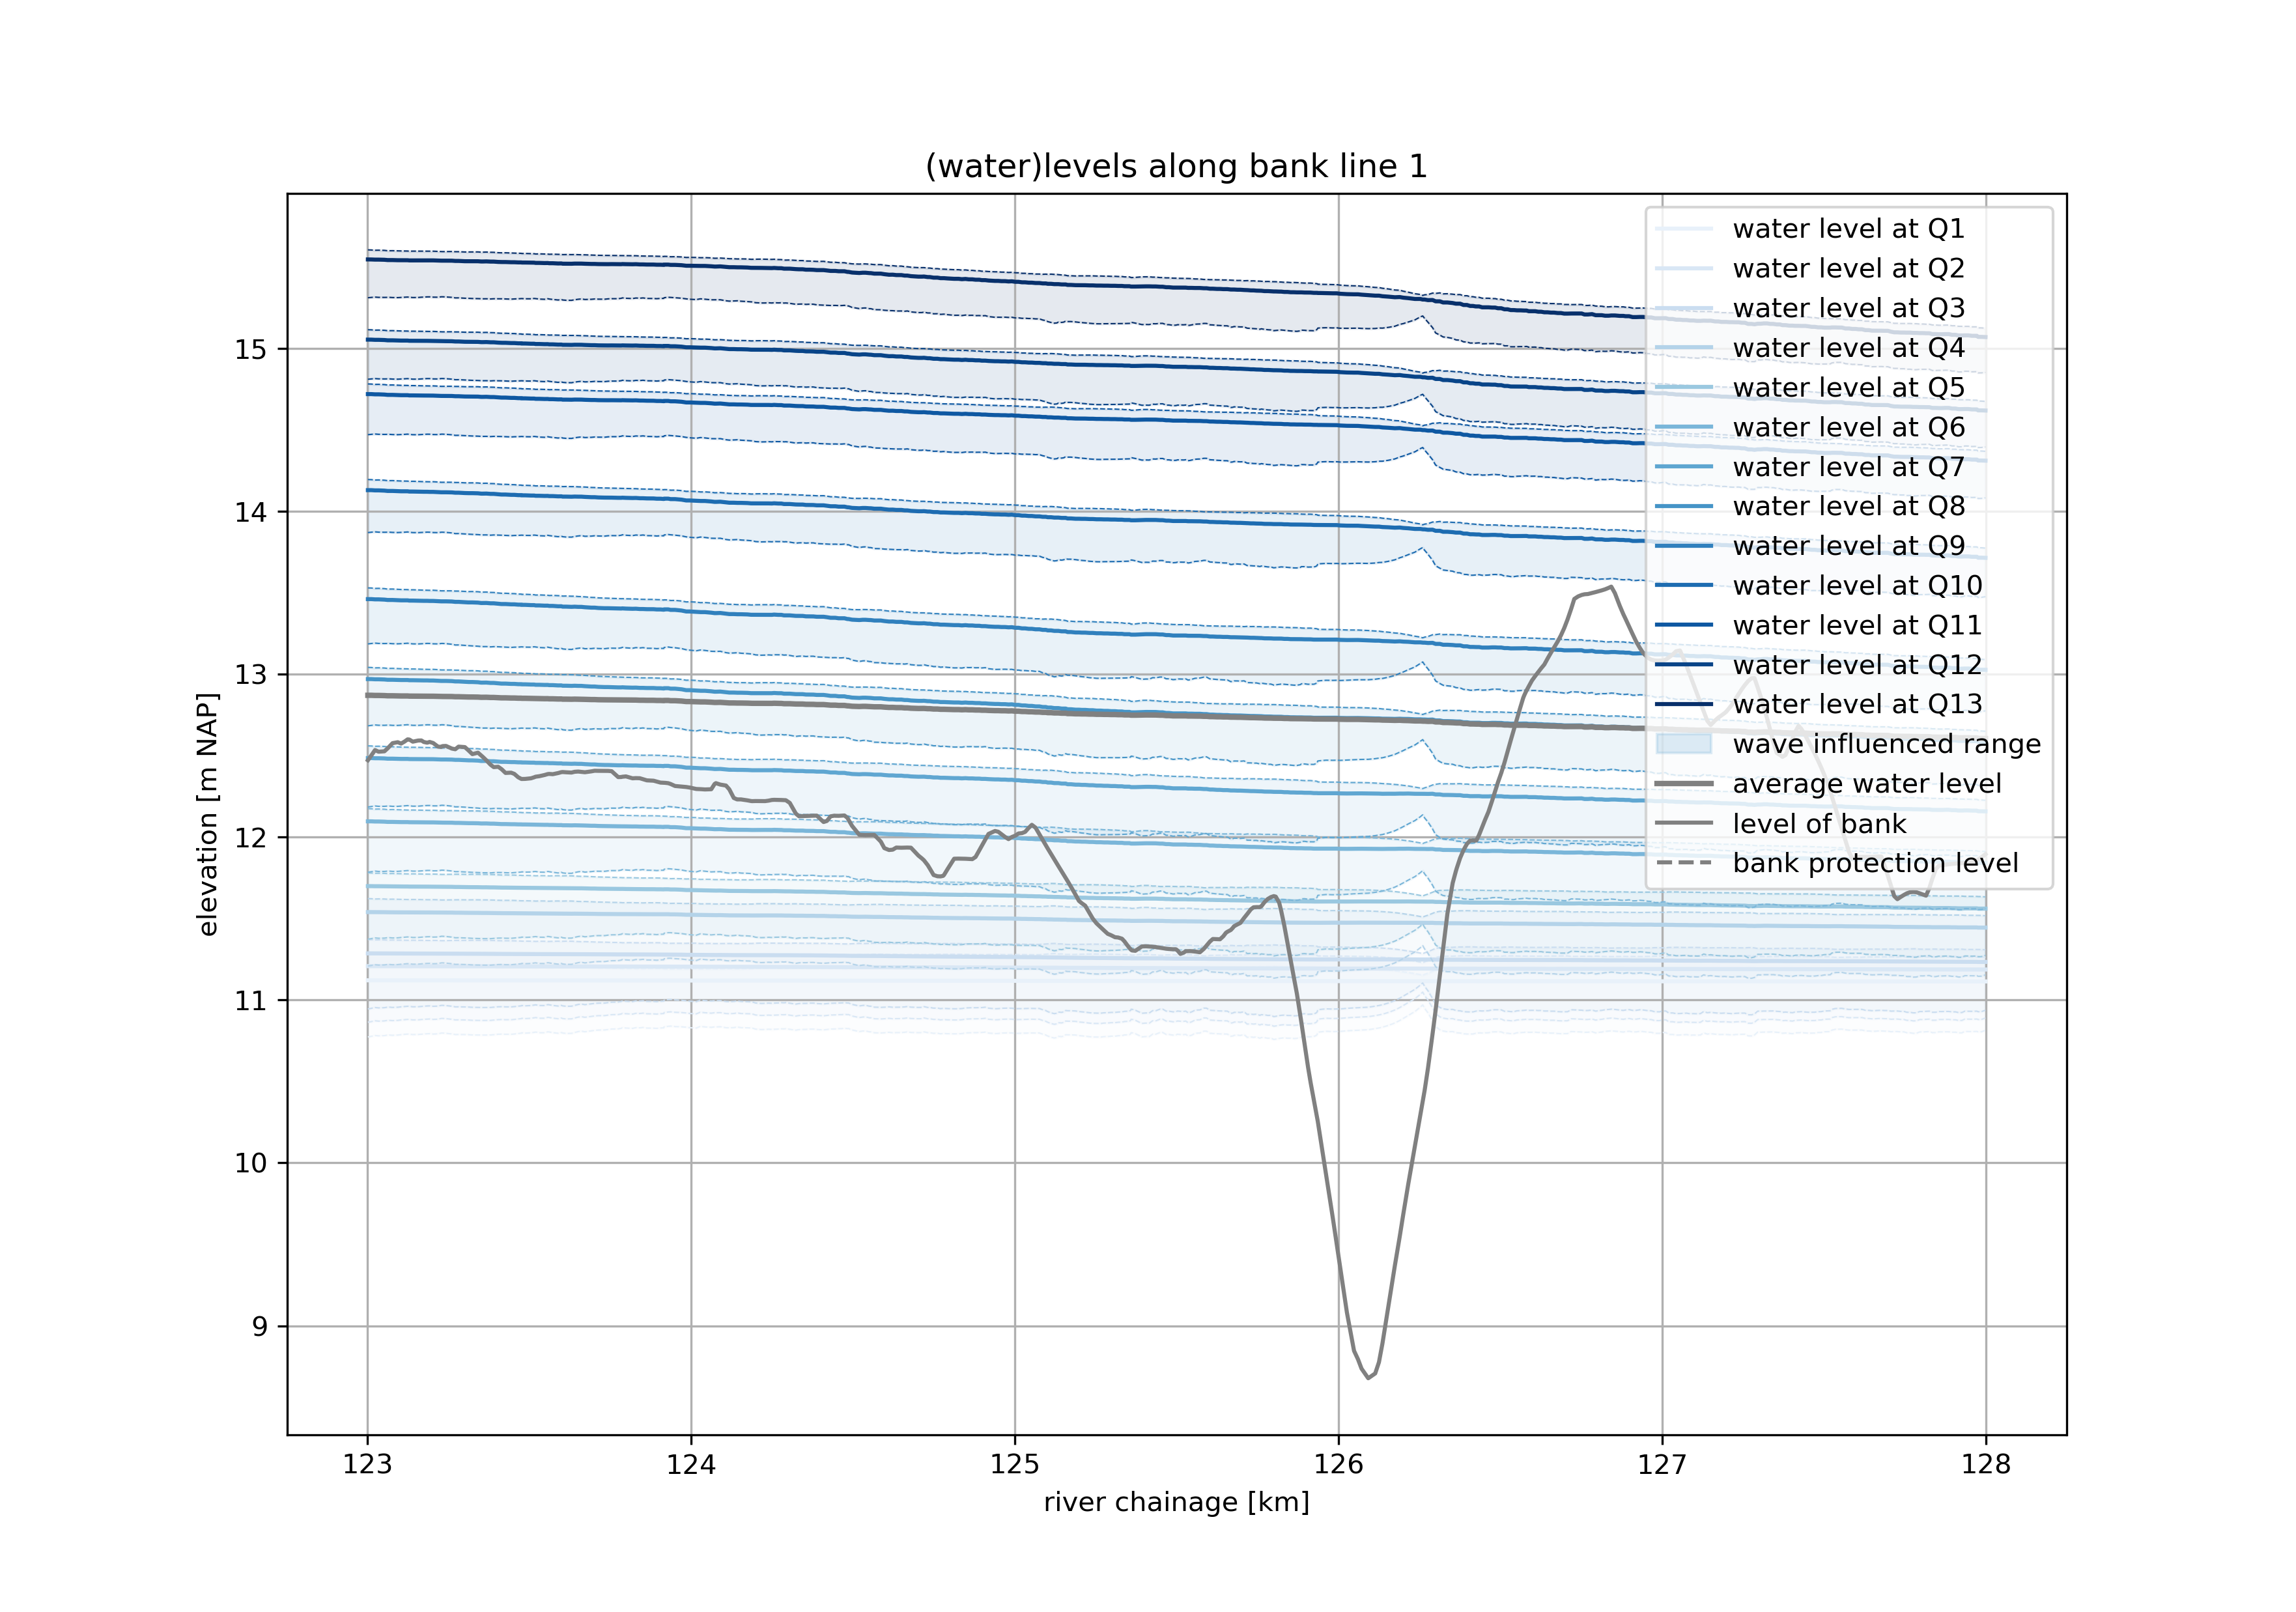
\includegraphics[width=\textwidth]{figures/6_levels_bank_1.png}
\caption{Control figure for water levels of each discharge (bank line 1)}
\label{Fig2.8}
\end{figure}
\clearpage
\begin{figure}
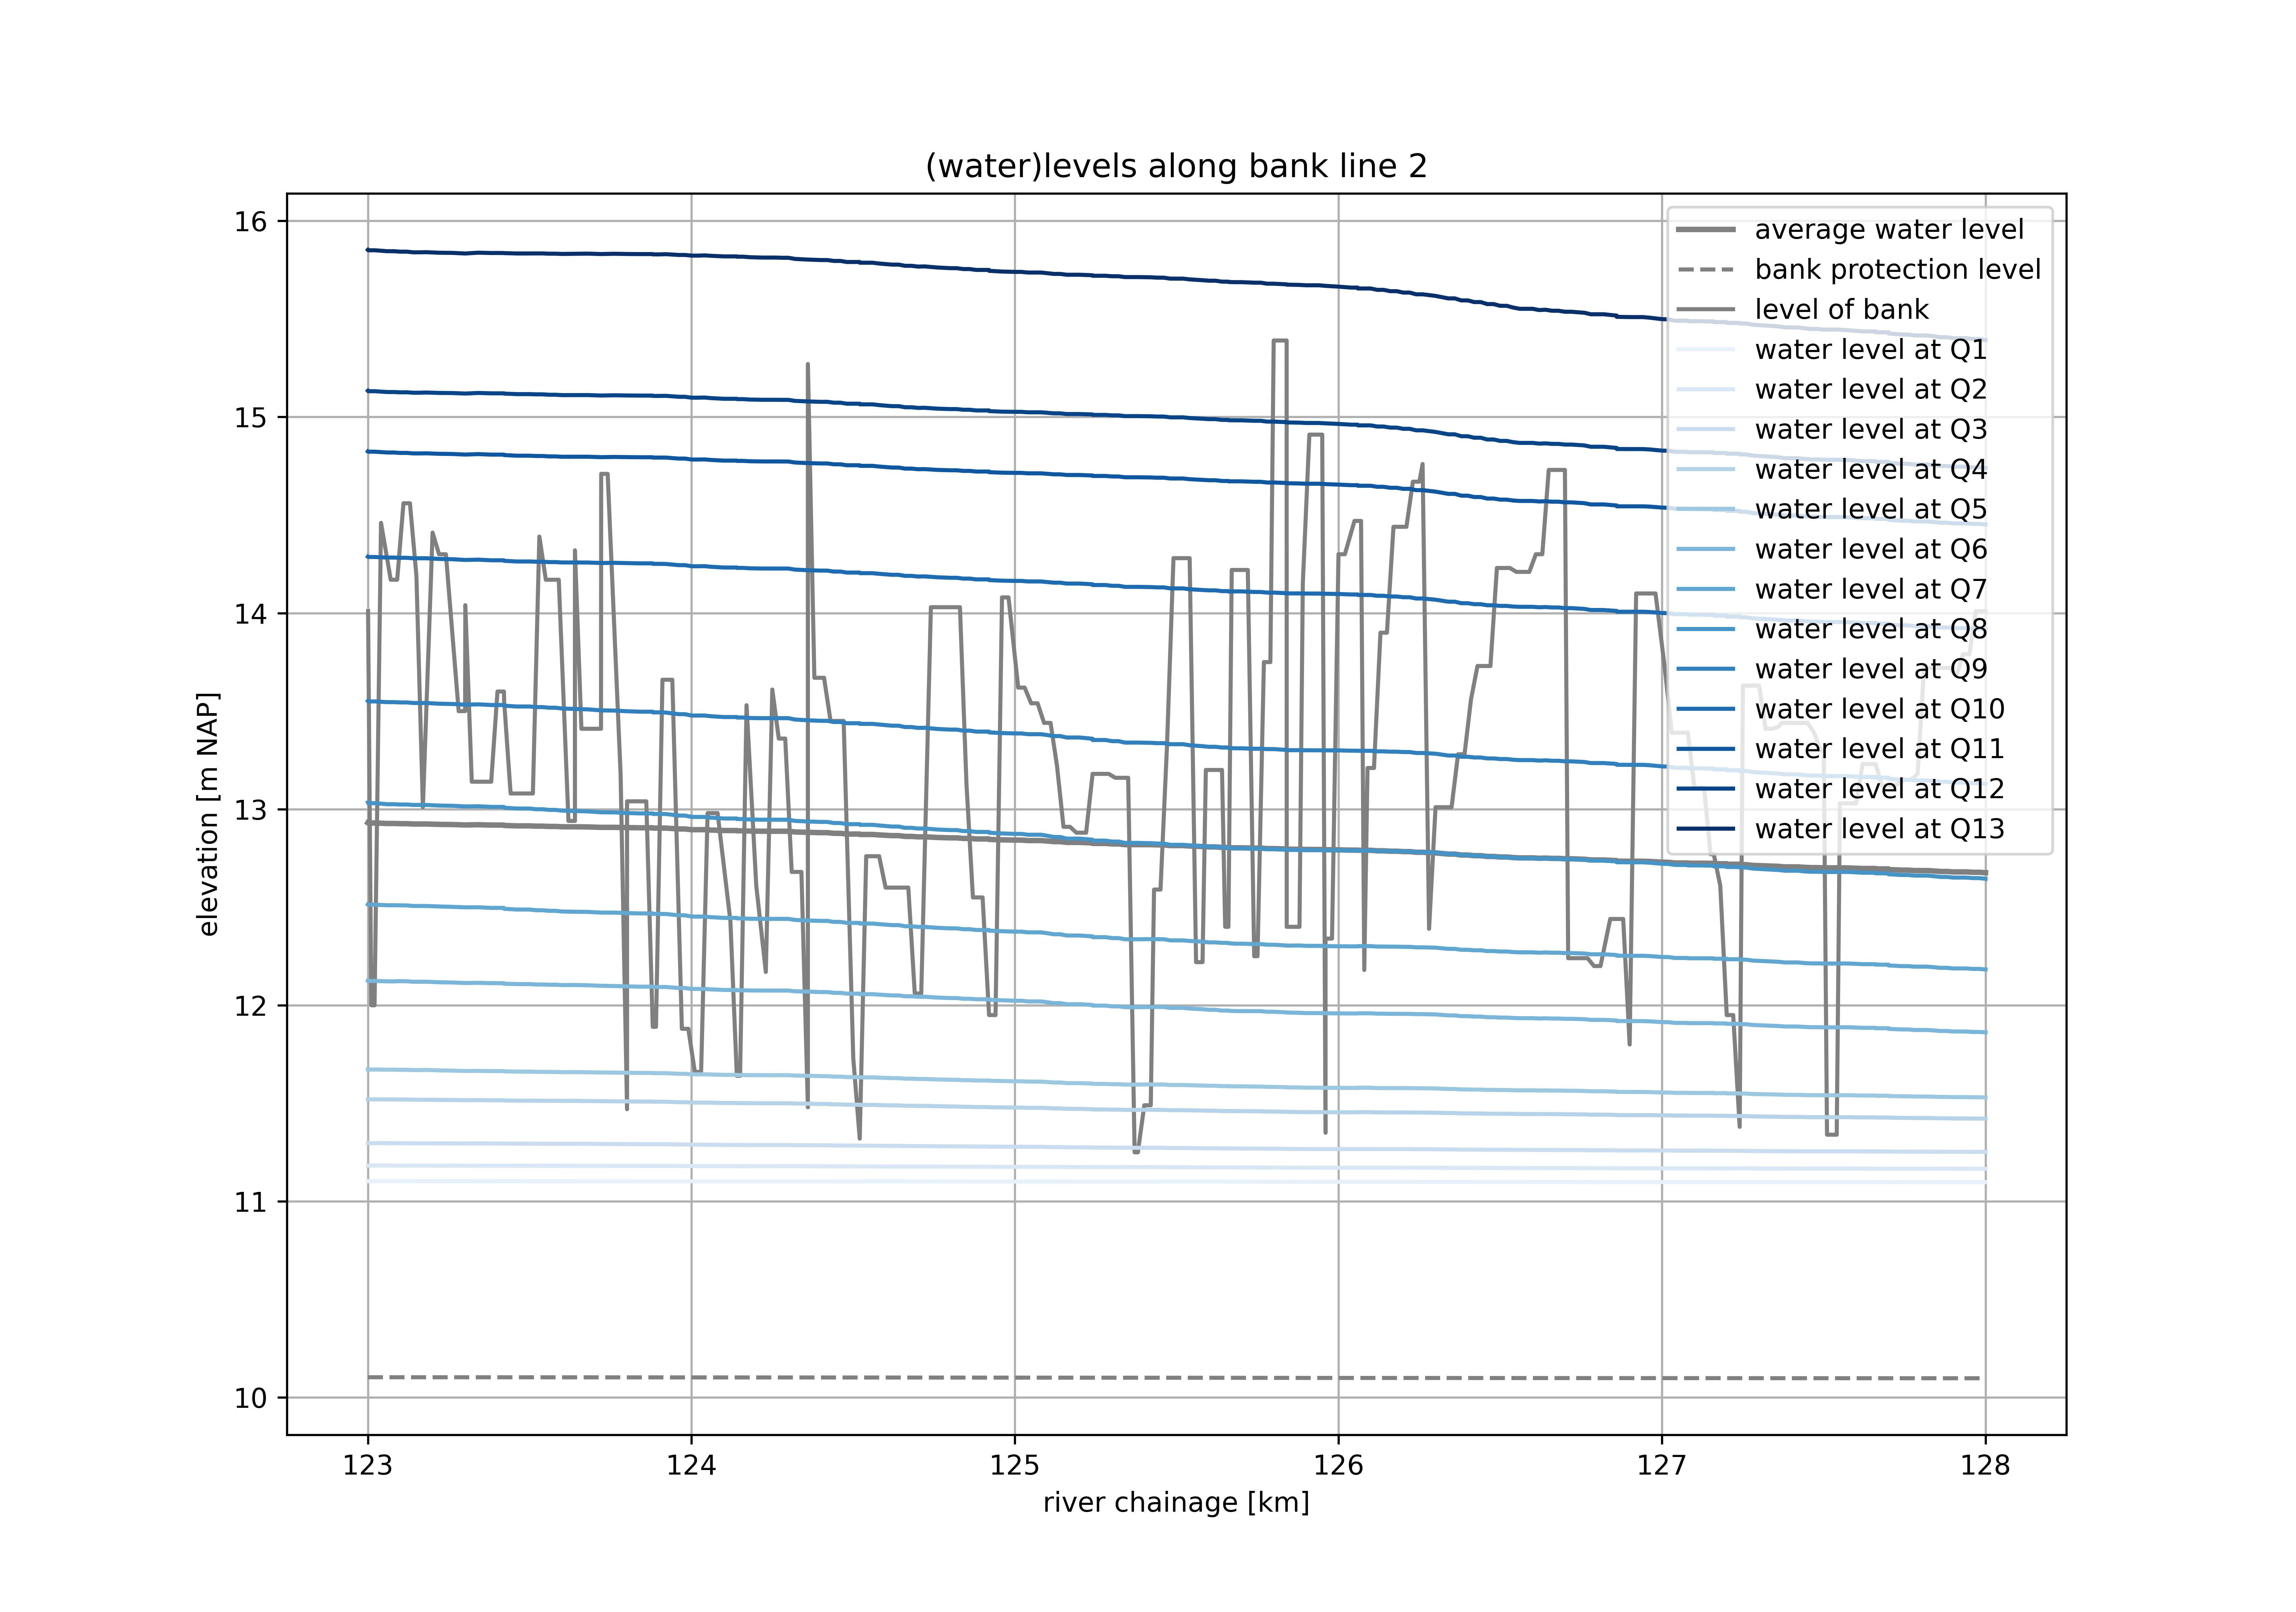
\includegraphics[width=\textwidth]{figures/7_levels_bank_2.png}
\caption{Control figure for water levels of each discharge (bank line 2)}
\label{Fig2.9}
\end{figure}

\begin{figure}
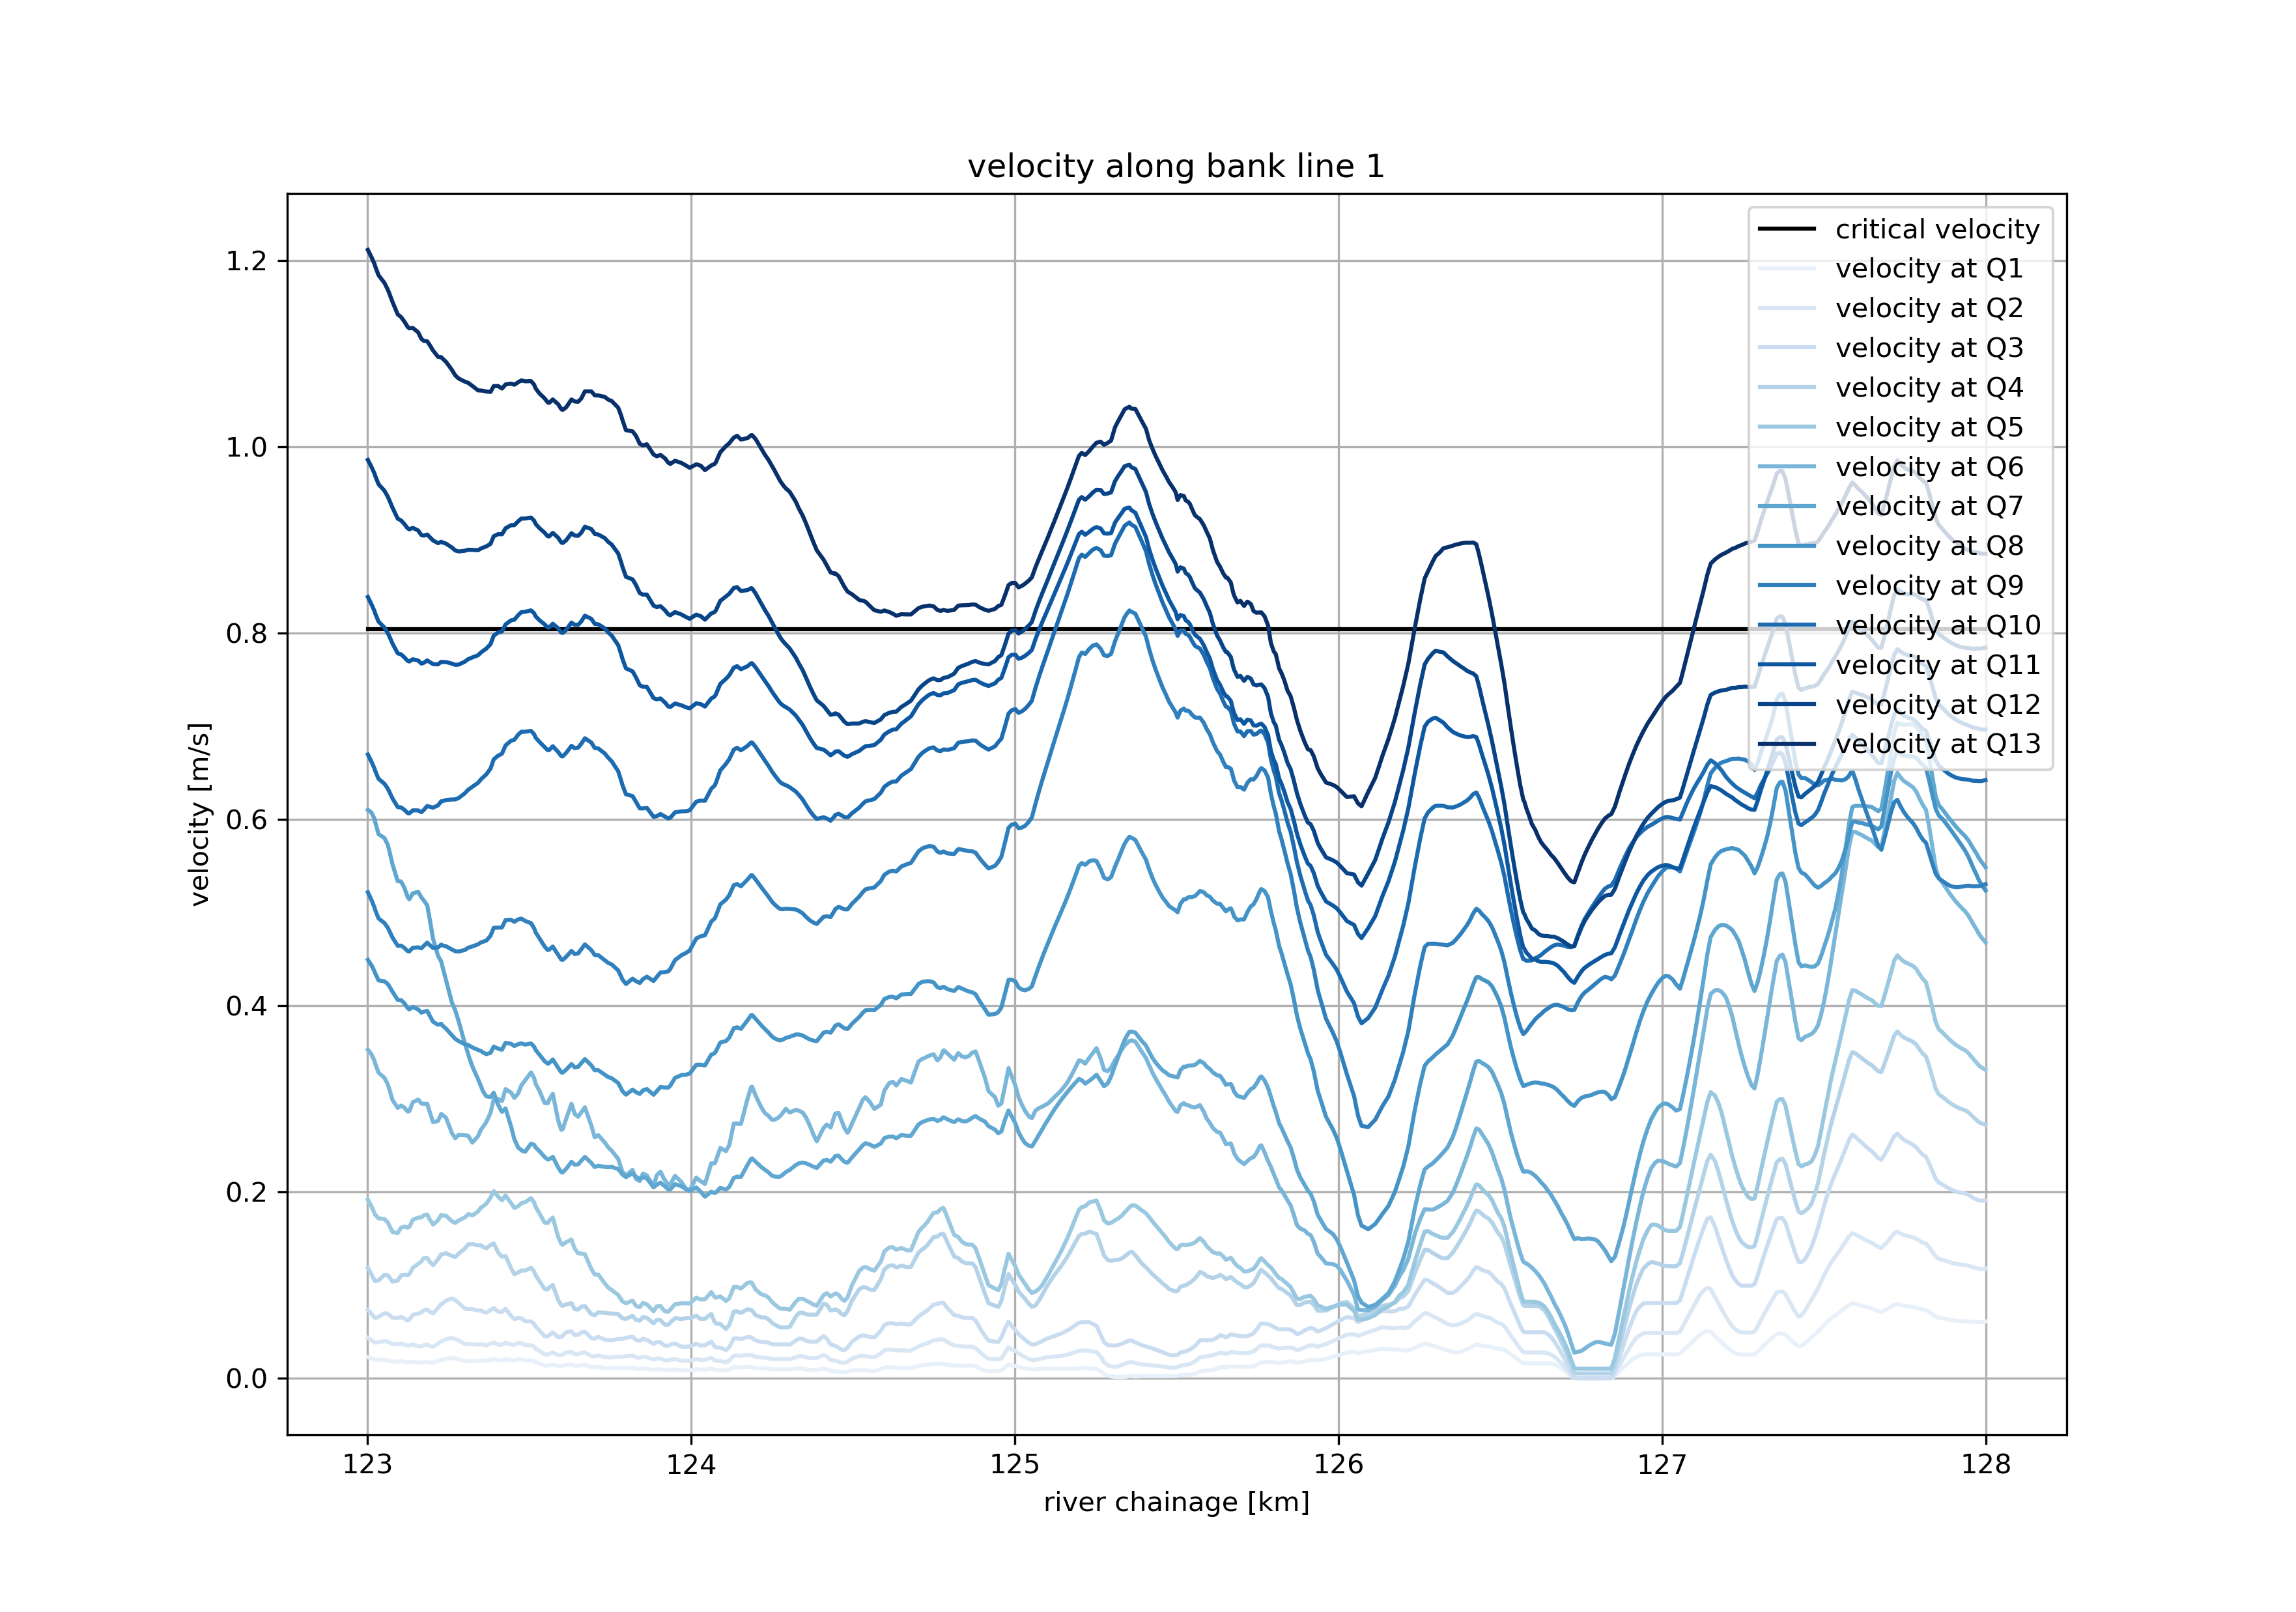
\includegraphics[width=\textwidth]{figures/8_velocity_bank_1.png}
\caption{Control figure for velocities of each discharge (bank line 1)}
\label{Fig2.10}
\end{figure}
\clearpage
\begin{figure}
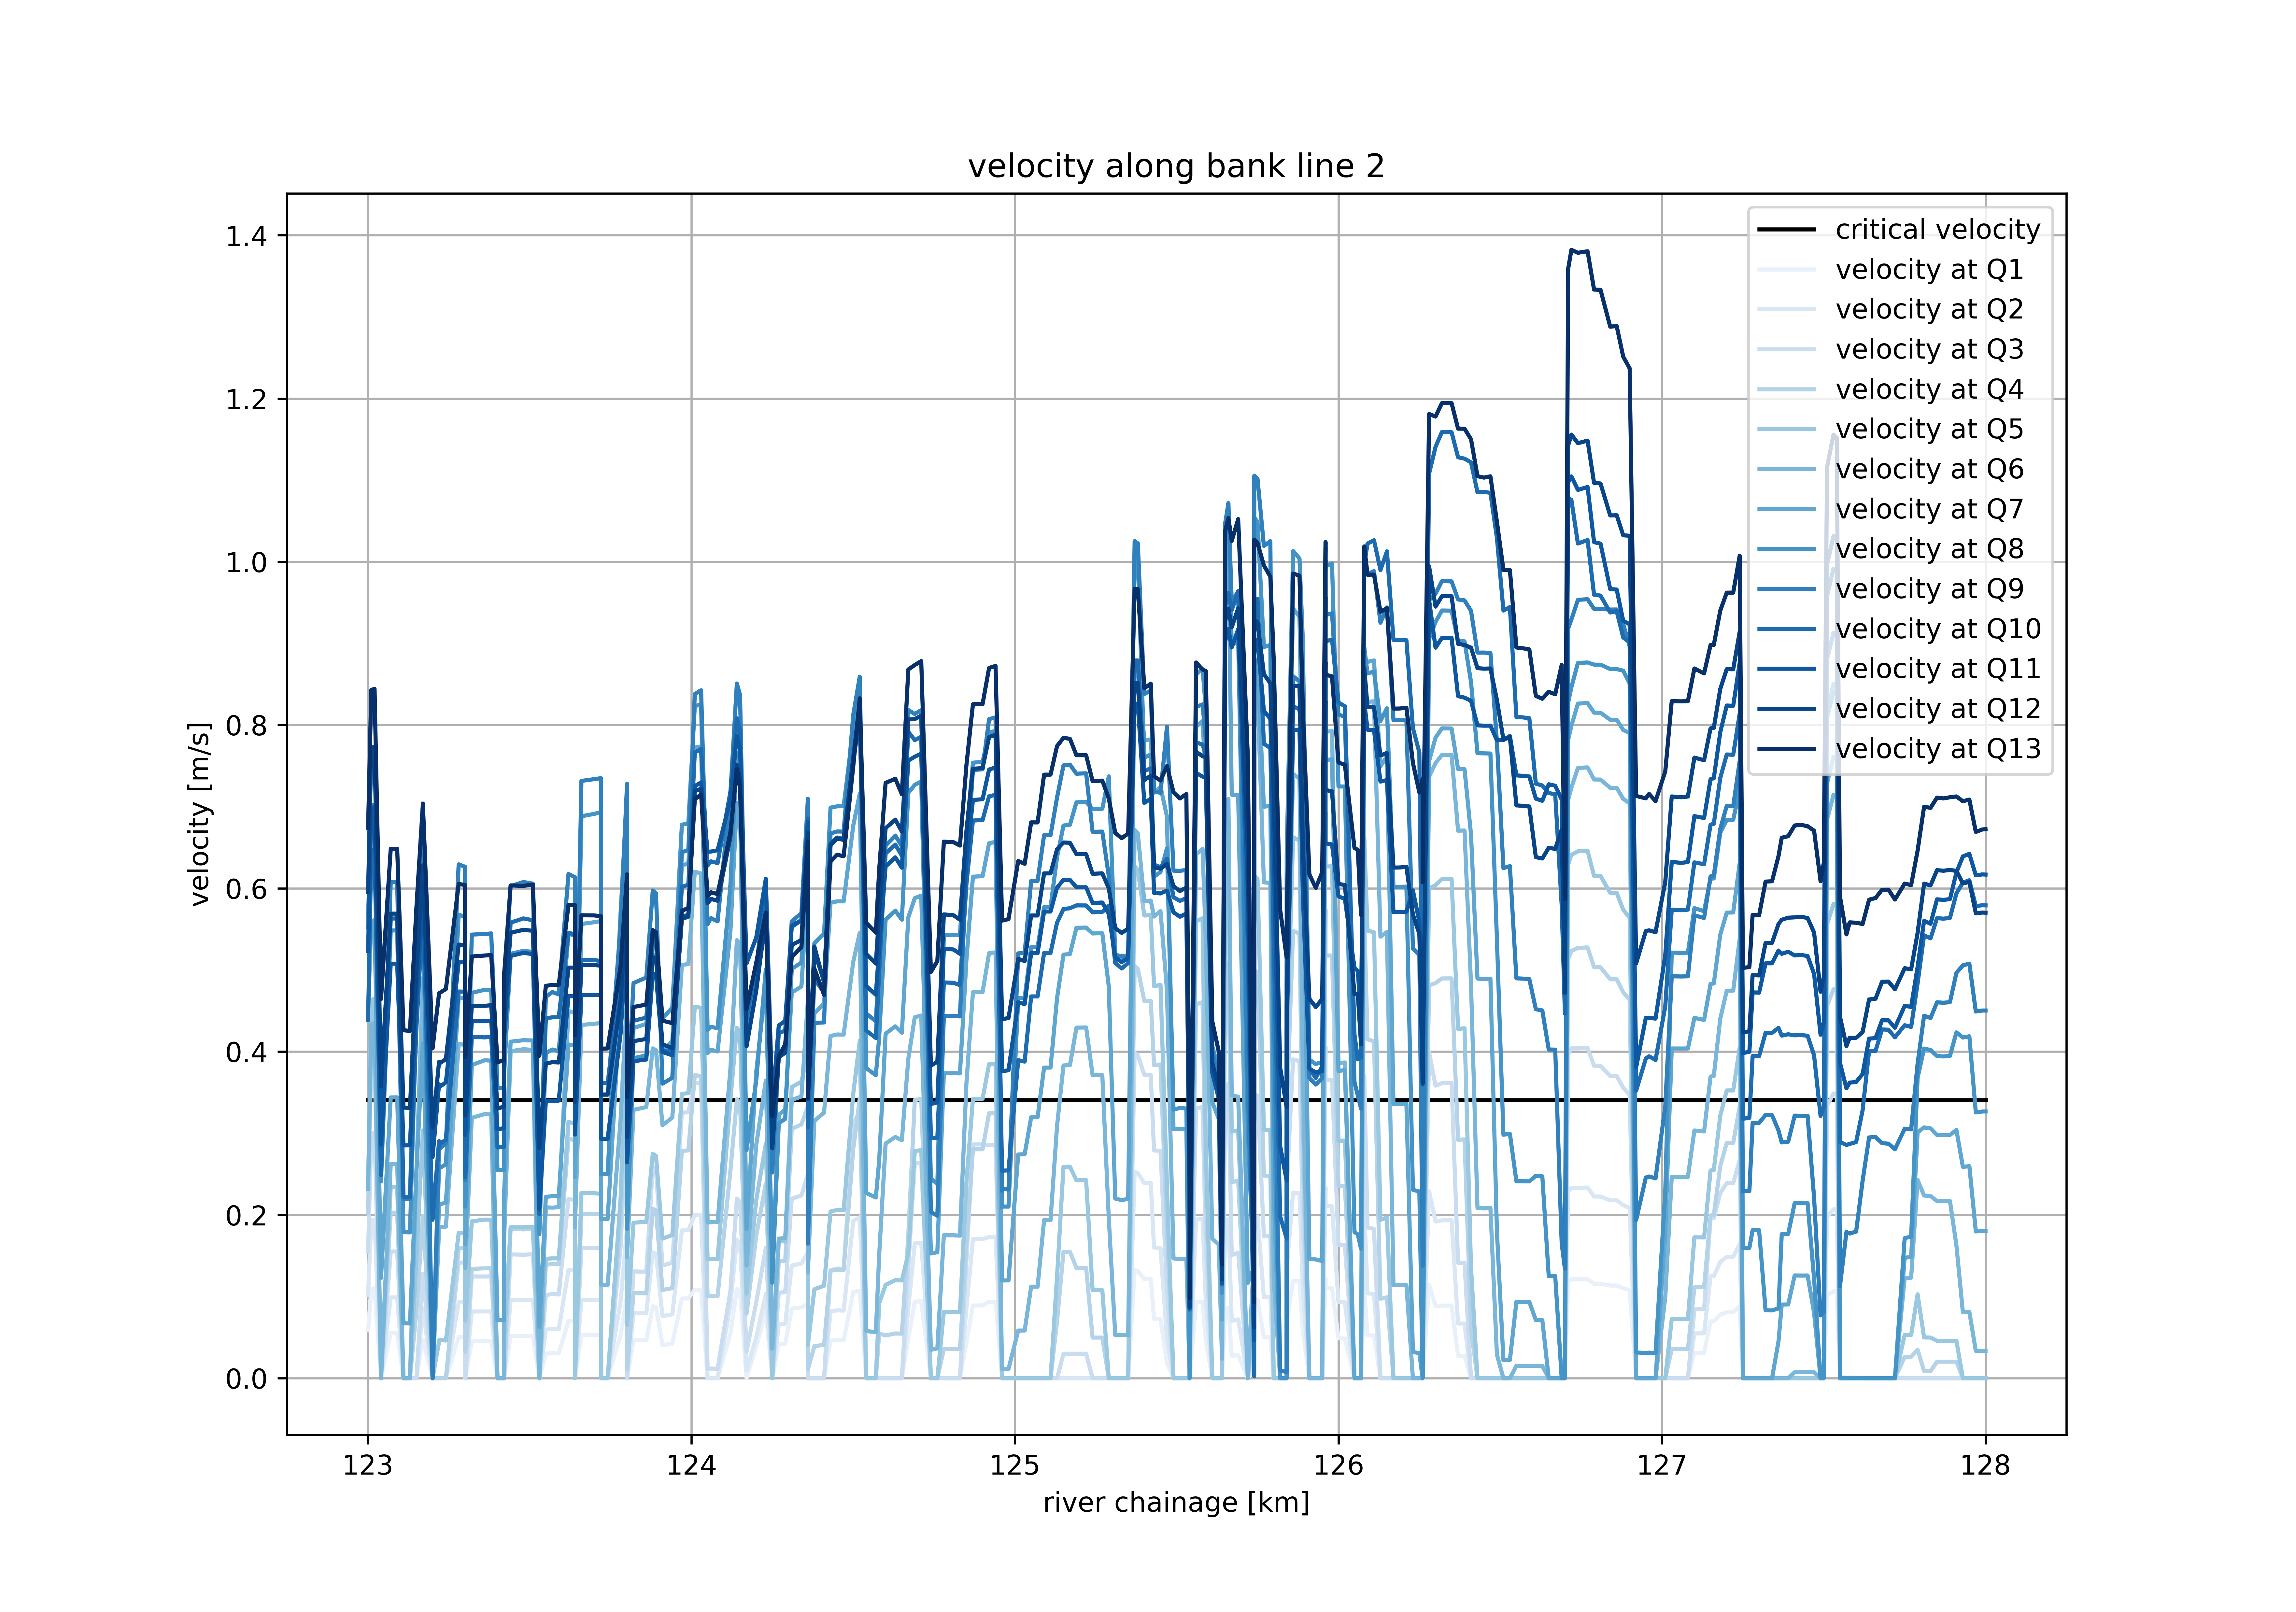
\includegraphics[width=\textwidth]{figures/9_velocity_bank_2.png}
\caption{Control figure for velocities of each discharge (bank line 2)}
\label{Fig2.11}
\end{figure}

\begin{figure}
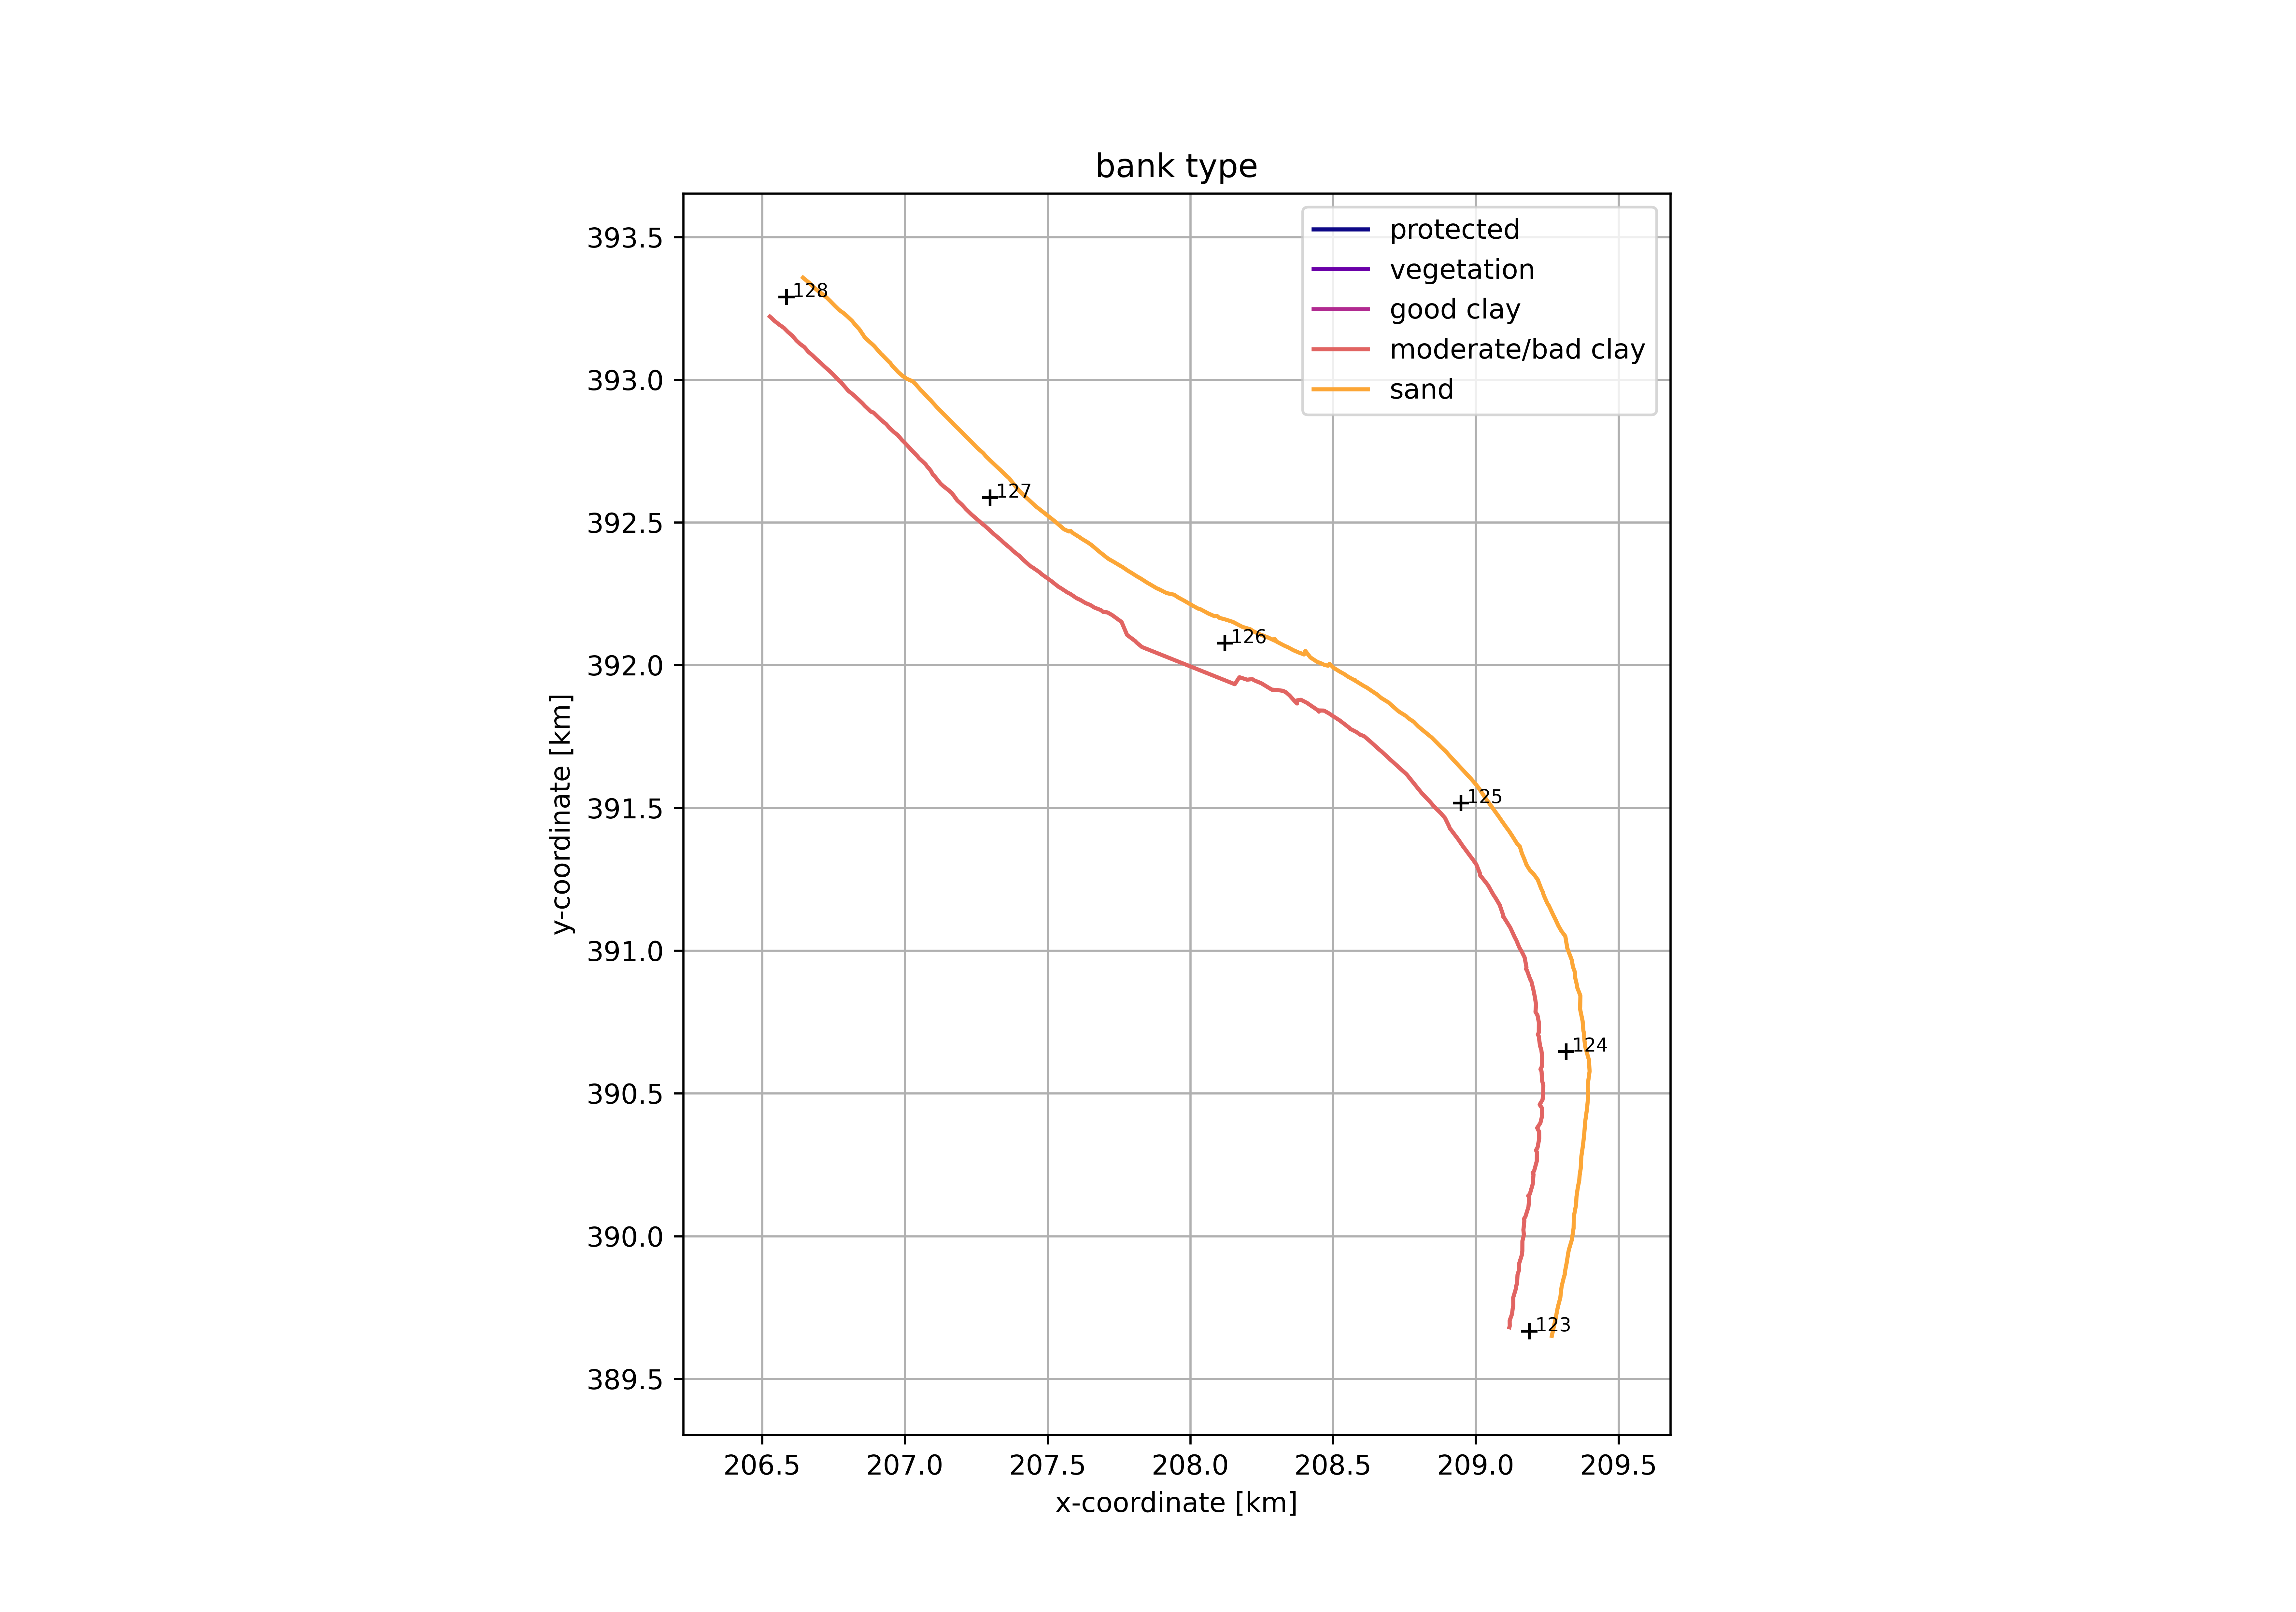
\includegraphics[width=\textwidth]{figures/10_banktype.png}
\caption{Map with indication of applied bank type}
\label{Fig2.12}
\end{figure}
\clearpage
\begin{figure}
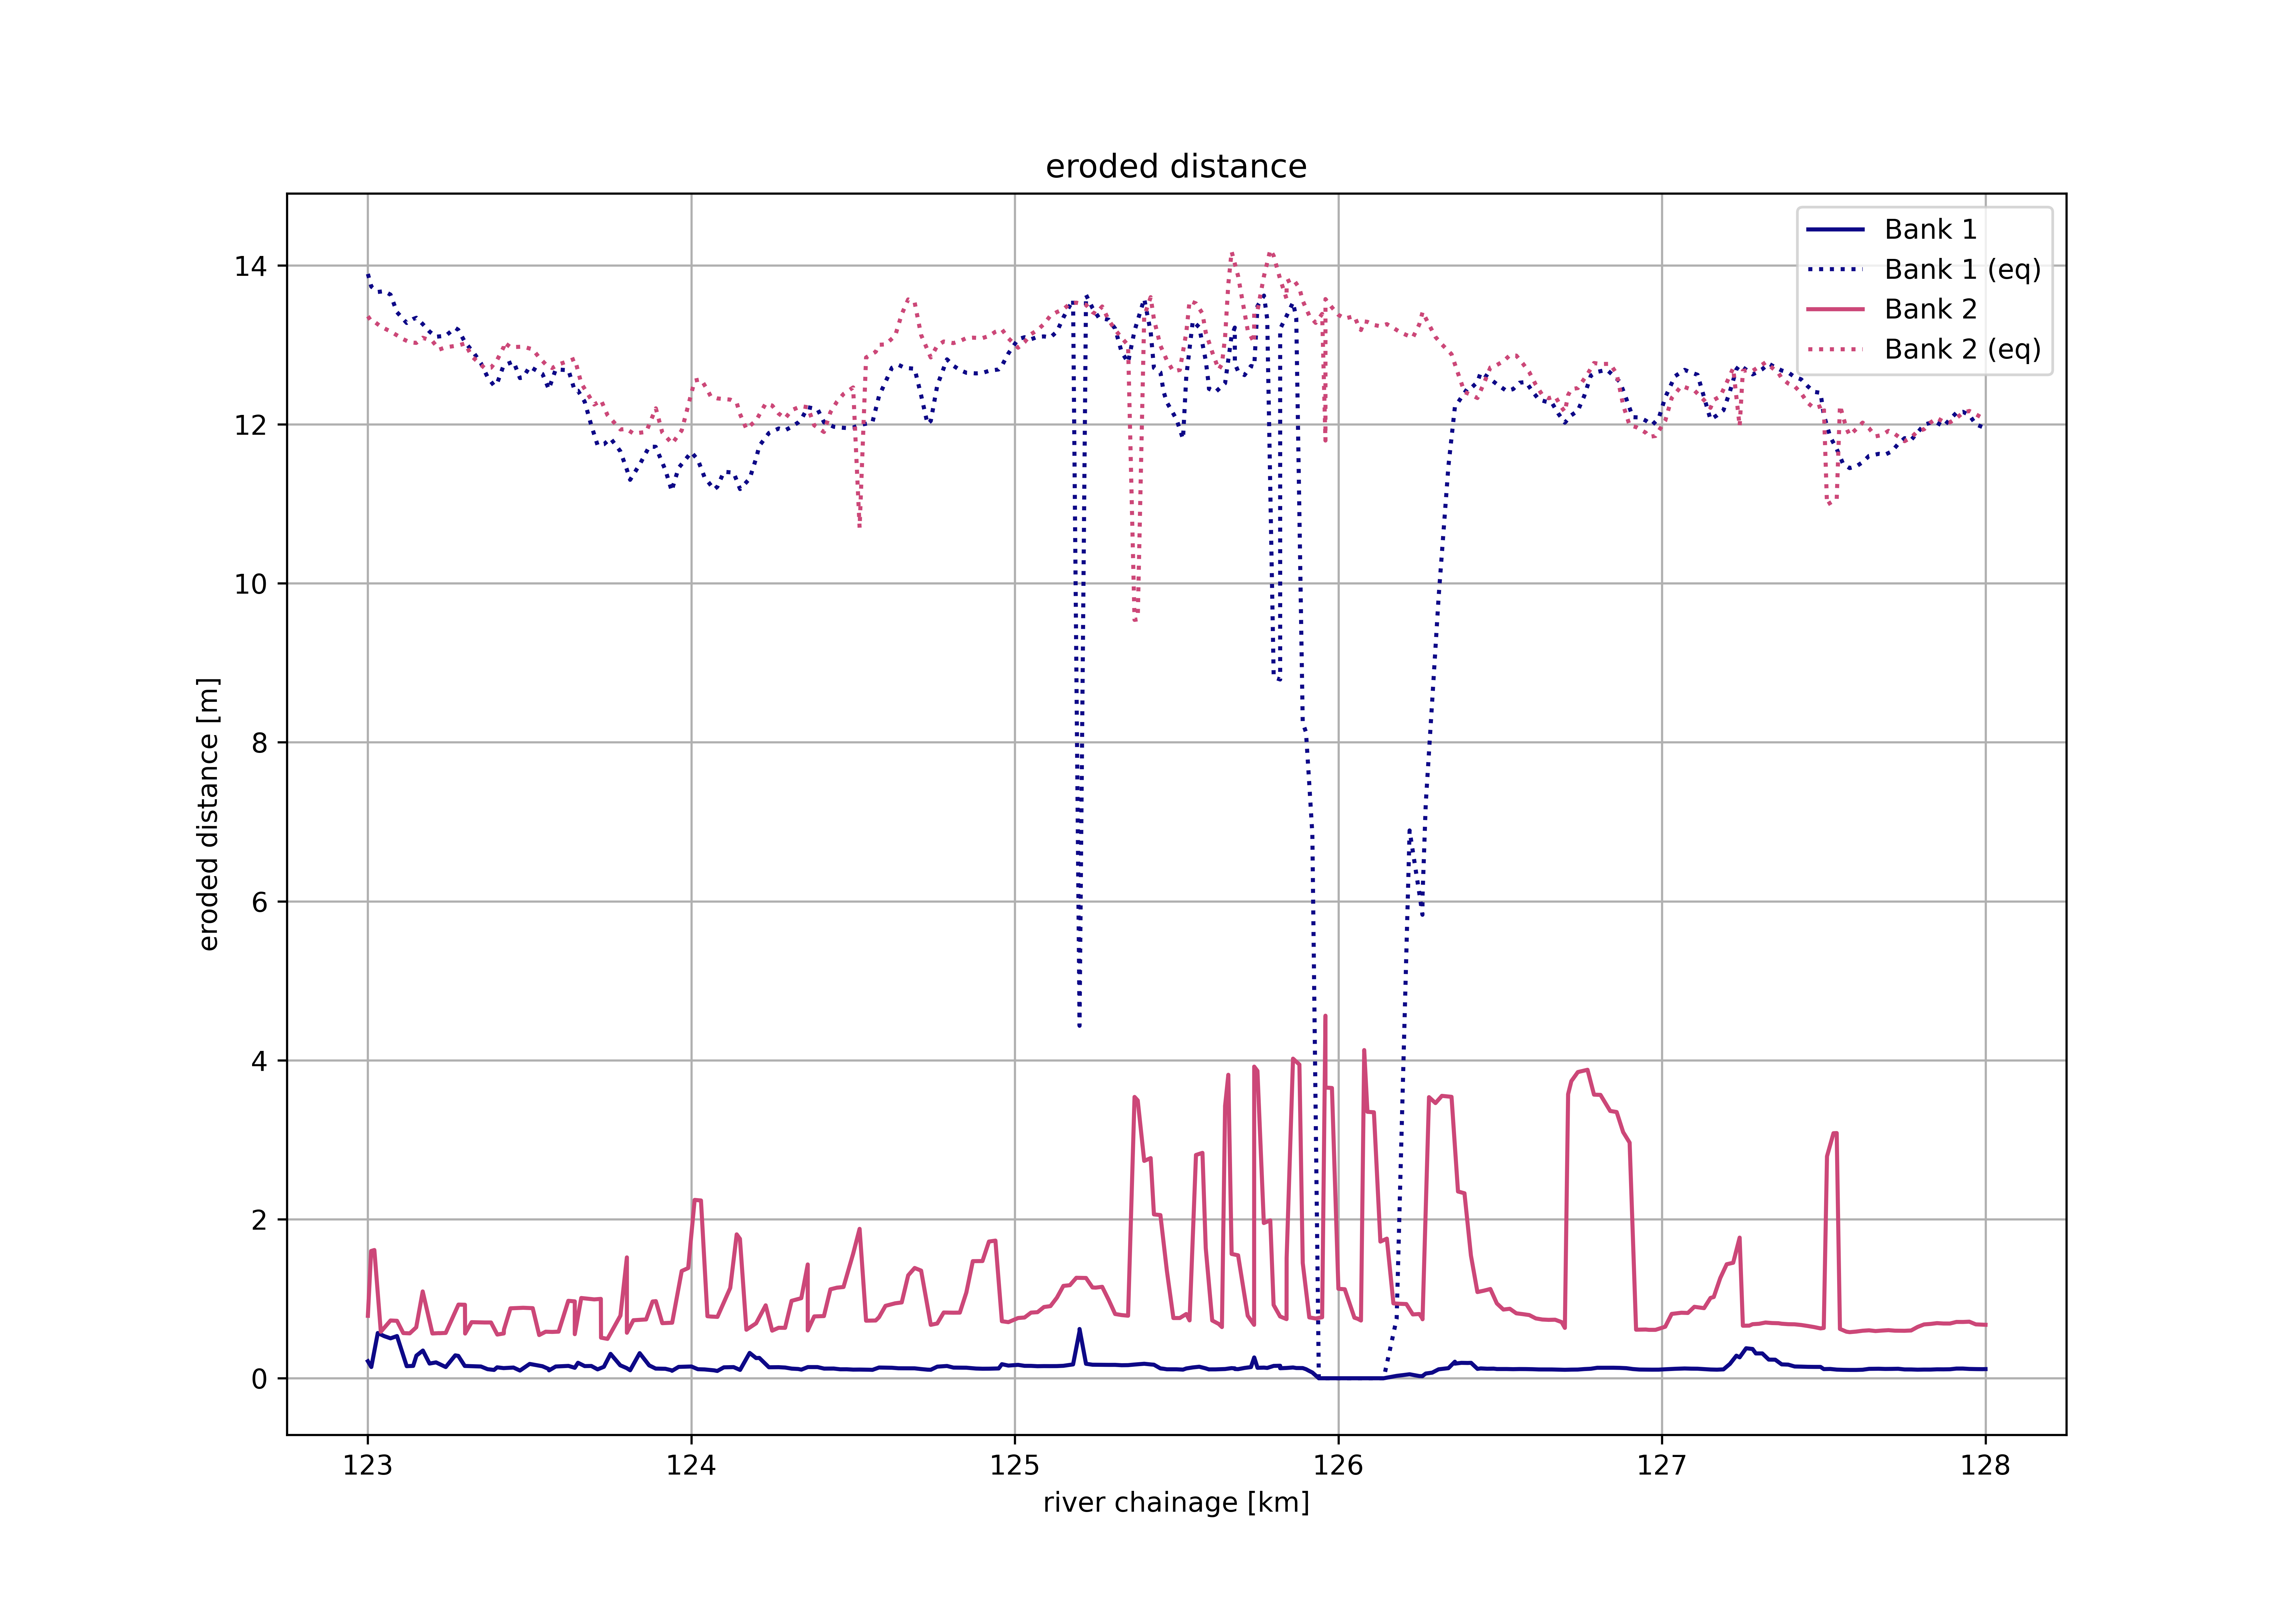
\includegraphics[width=\textwidth]{figures/11_erodis.png}
\caption{Bank retreat at the end of the simulation period and for the equilibrium situation}
\label{Fig2.13}
\end{figure}

\section{Running from Python source code} \label{Sec:Python}
\dfastbe can also be run directly from the Python source code.
For this you will need to download the source code as well as the correct version of several third party modules used by the tool.
Please check the \dfastbe Technical Reference manual for details.
When running the tool from Python source code, the program can be started from the command prompt as

\begin{Verbatim}
python -m dfastbe ...options...
\end{Verbatim}

or from within a running Python environment as

\begin{Verbatim}
import dfastbe.cmd
dfastbe.cmd.run()
\end{Verbatim}

where optionally the \command{language} (default \command{UK}), \command{runmode} (default \command{GUI}) and \command{configfile} (default \command{dfastbe.cfg}) can be specified as arguments.